\chapter[Data Transformations]{Data Transformations: Two Philosophies on Hydrologic Processes} \label{ch2:transformations}
\chaptermark{Data Transformations}
\setlength{\epigraphwidth}{4.5in}
\epigraph{Science is what we know, and philosophy is what we don't know.}{Bertrand Russell, \textit{``Unpopular Essays''}, 1950}

%----------------------------------------------------------------------------------------------------------------------------------------------------------------------------------------------------------
\section*{Summary}
This chapter developed linear multivariate regression (LM), generalized linear regression (GLM), random forest (RF), and Neural Network (NN) models with a typical least squares loss function, of monthly unimpaired flows in 67 California basins. The best overall error (Bias-Corrected Coefficient of Determination, bR\textsuperscript{2}=0.92, Nash-Sutcliffe Efficiency, NSE=0.97) reflects the model's ability to capture monthly variations in flow. The NN with ``incremental basins" performed the best in the NSE criterion. Incremental basins are segments of the basin that have not been gauged, a concept discussed in this chapter. 

The test set error from ``leave one group out" (LOGO) cross-validation shows that model quality in predicting unimpaired flow is very spatially variable. LOGO cross validation and other resampling strategies are discussed in the next chapter. A comparison of different models concludes that the incremental basin approach to hydrologic modeling provides increasing benefits as the outlet of interest moves downstream in the gauge network. 

%Lastly, next steps and model improvement strategies are discussed.

%----------------------------------------------------------------------------------------------------------------------------------------------------------------------------------------------------------
\section{Introduction}
% add literature review here: klemes on double mass curves, 1922 varletes res opt, ripple method
%what is this chapter about, practical problems, literature, major contributions and structure
Unimpaired flows can be presented in two fundamentally different ways: (1) we can imagine each basin as a separate function that transforms its inputs (precipitation and snow) into runoff (or unimpaired stream flow). Here, we define each basin to be an ``aggregate" basin. Flows for these basins are simply the observed gauge values (Figure \ref{fig:aggbasins}); (2) we can imagine the basins as interconnected, and overlapping. One stream flows into another, like in a network, and so, some basins overlap. Here, we can define ``incremental" basins to be segments of basins that do not overlap. Flows for these basins are the amount that has not been observed by gauges in the network above the outlet of interest (Figure \ref{fig:incbasins}). Therefore, when modeling incremental flows, the network information is being preserved.

%\begin{figure}
%	\centering
%	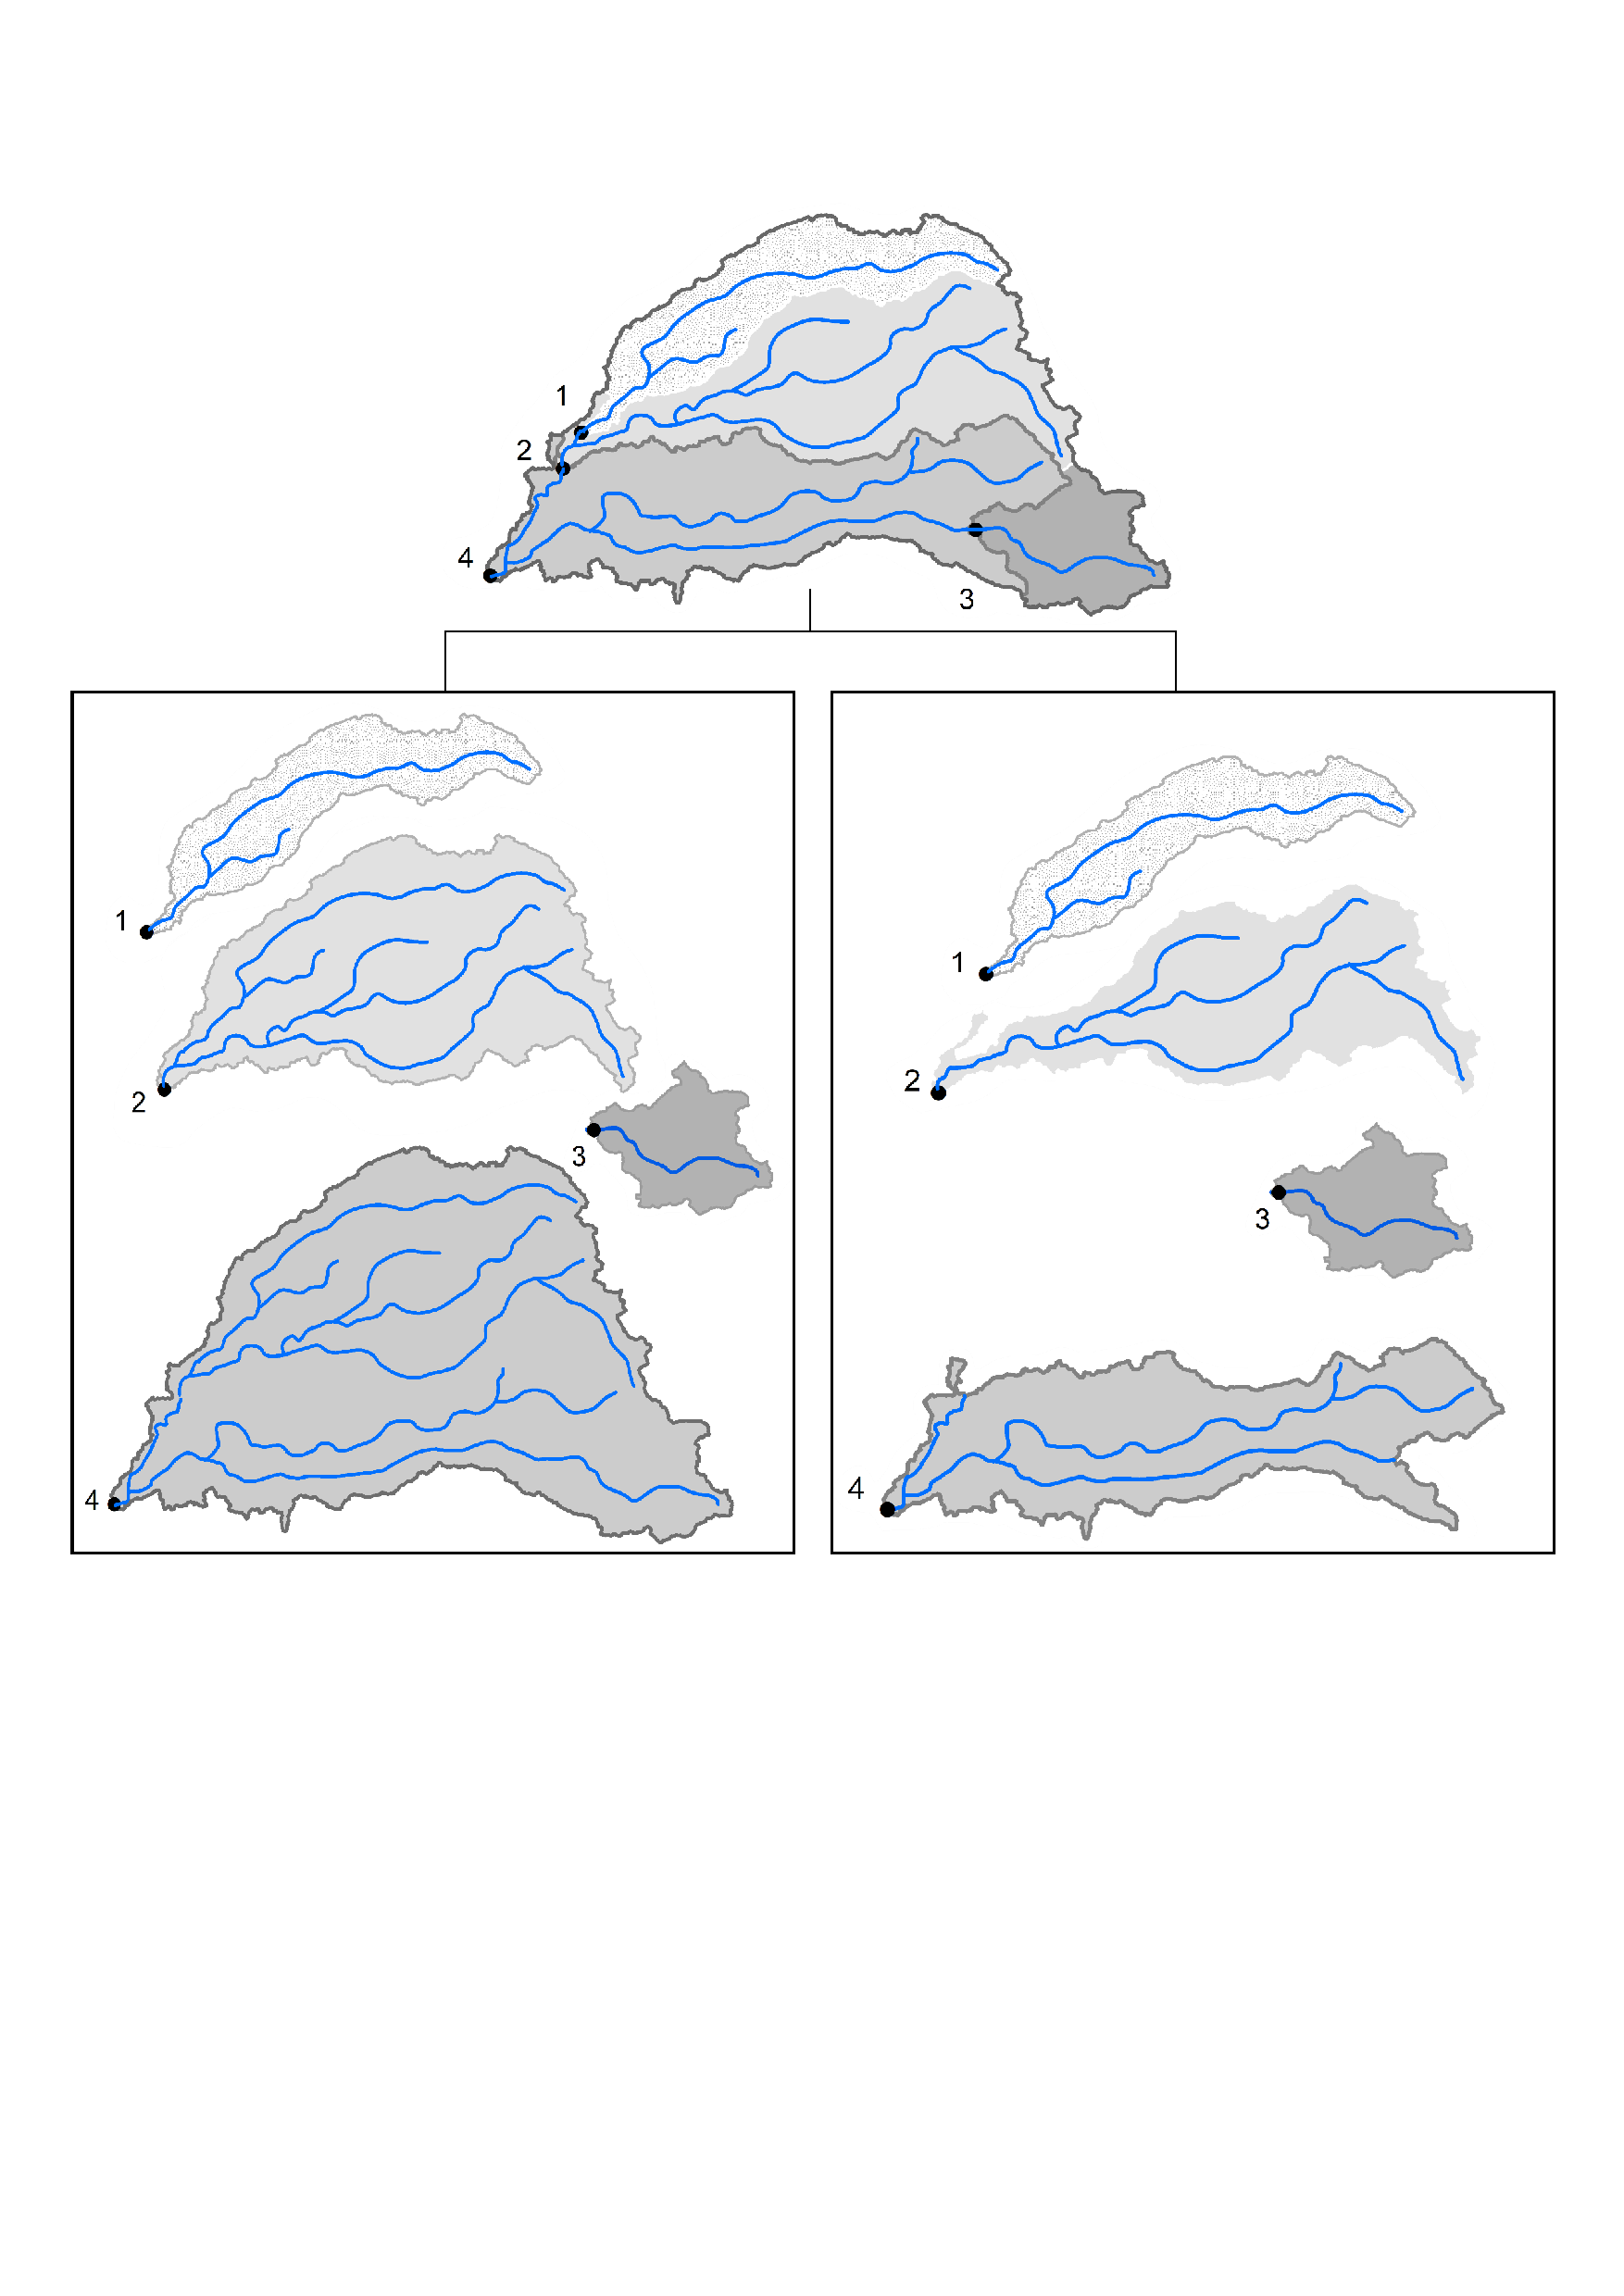
\includegraphics[width=16.5cm,trim={0 10cm 0 3cm},clip=true]{plots/agg_and_inc_basins.pdf}
%	\caption{Agg and Inc Basins} 
%	\label{fig:aggincbasins}
%\end{figure}

\begin{figure}
	\centering
	\begin{subfigure}{0.7\textwidth}
  		\centering
 		 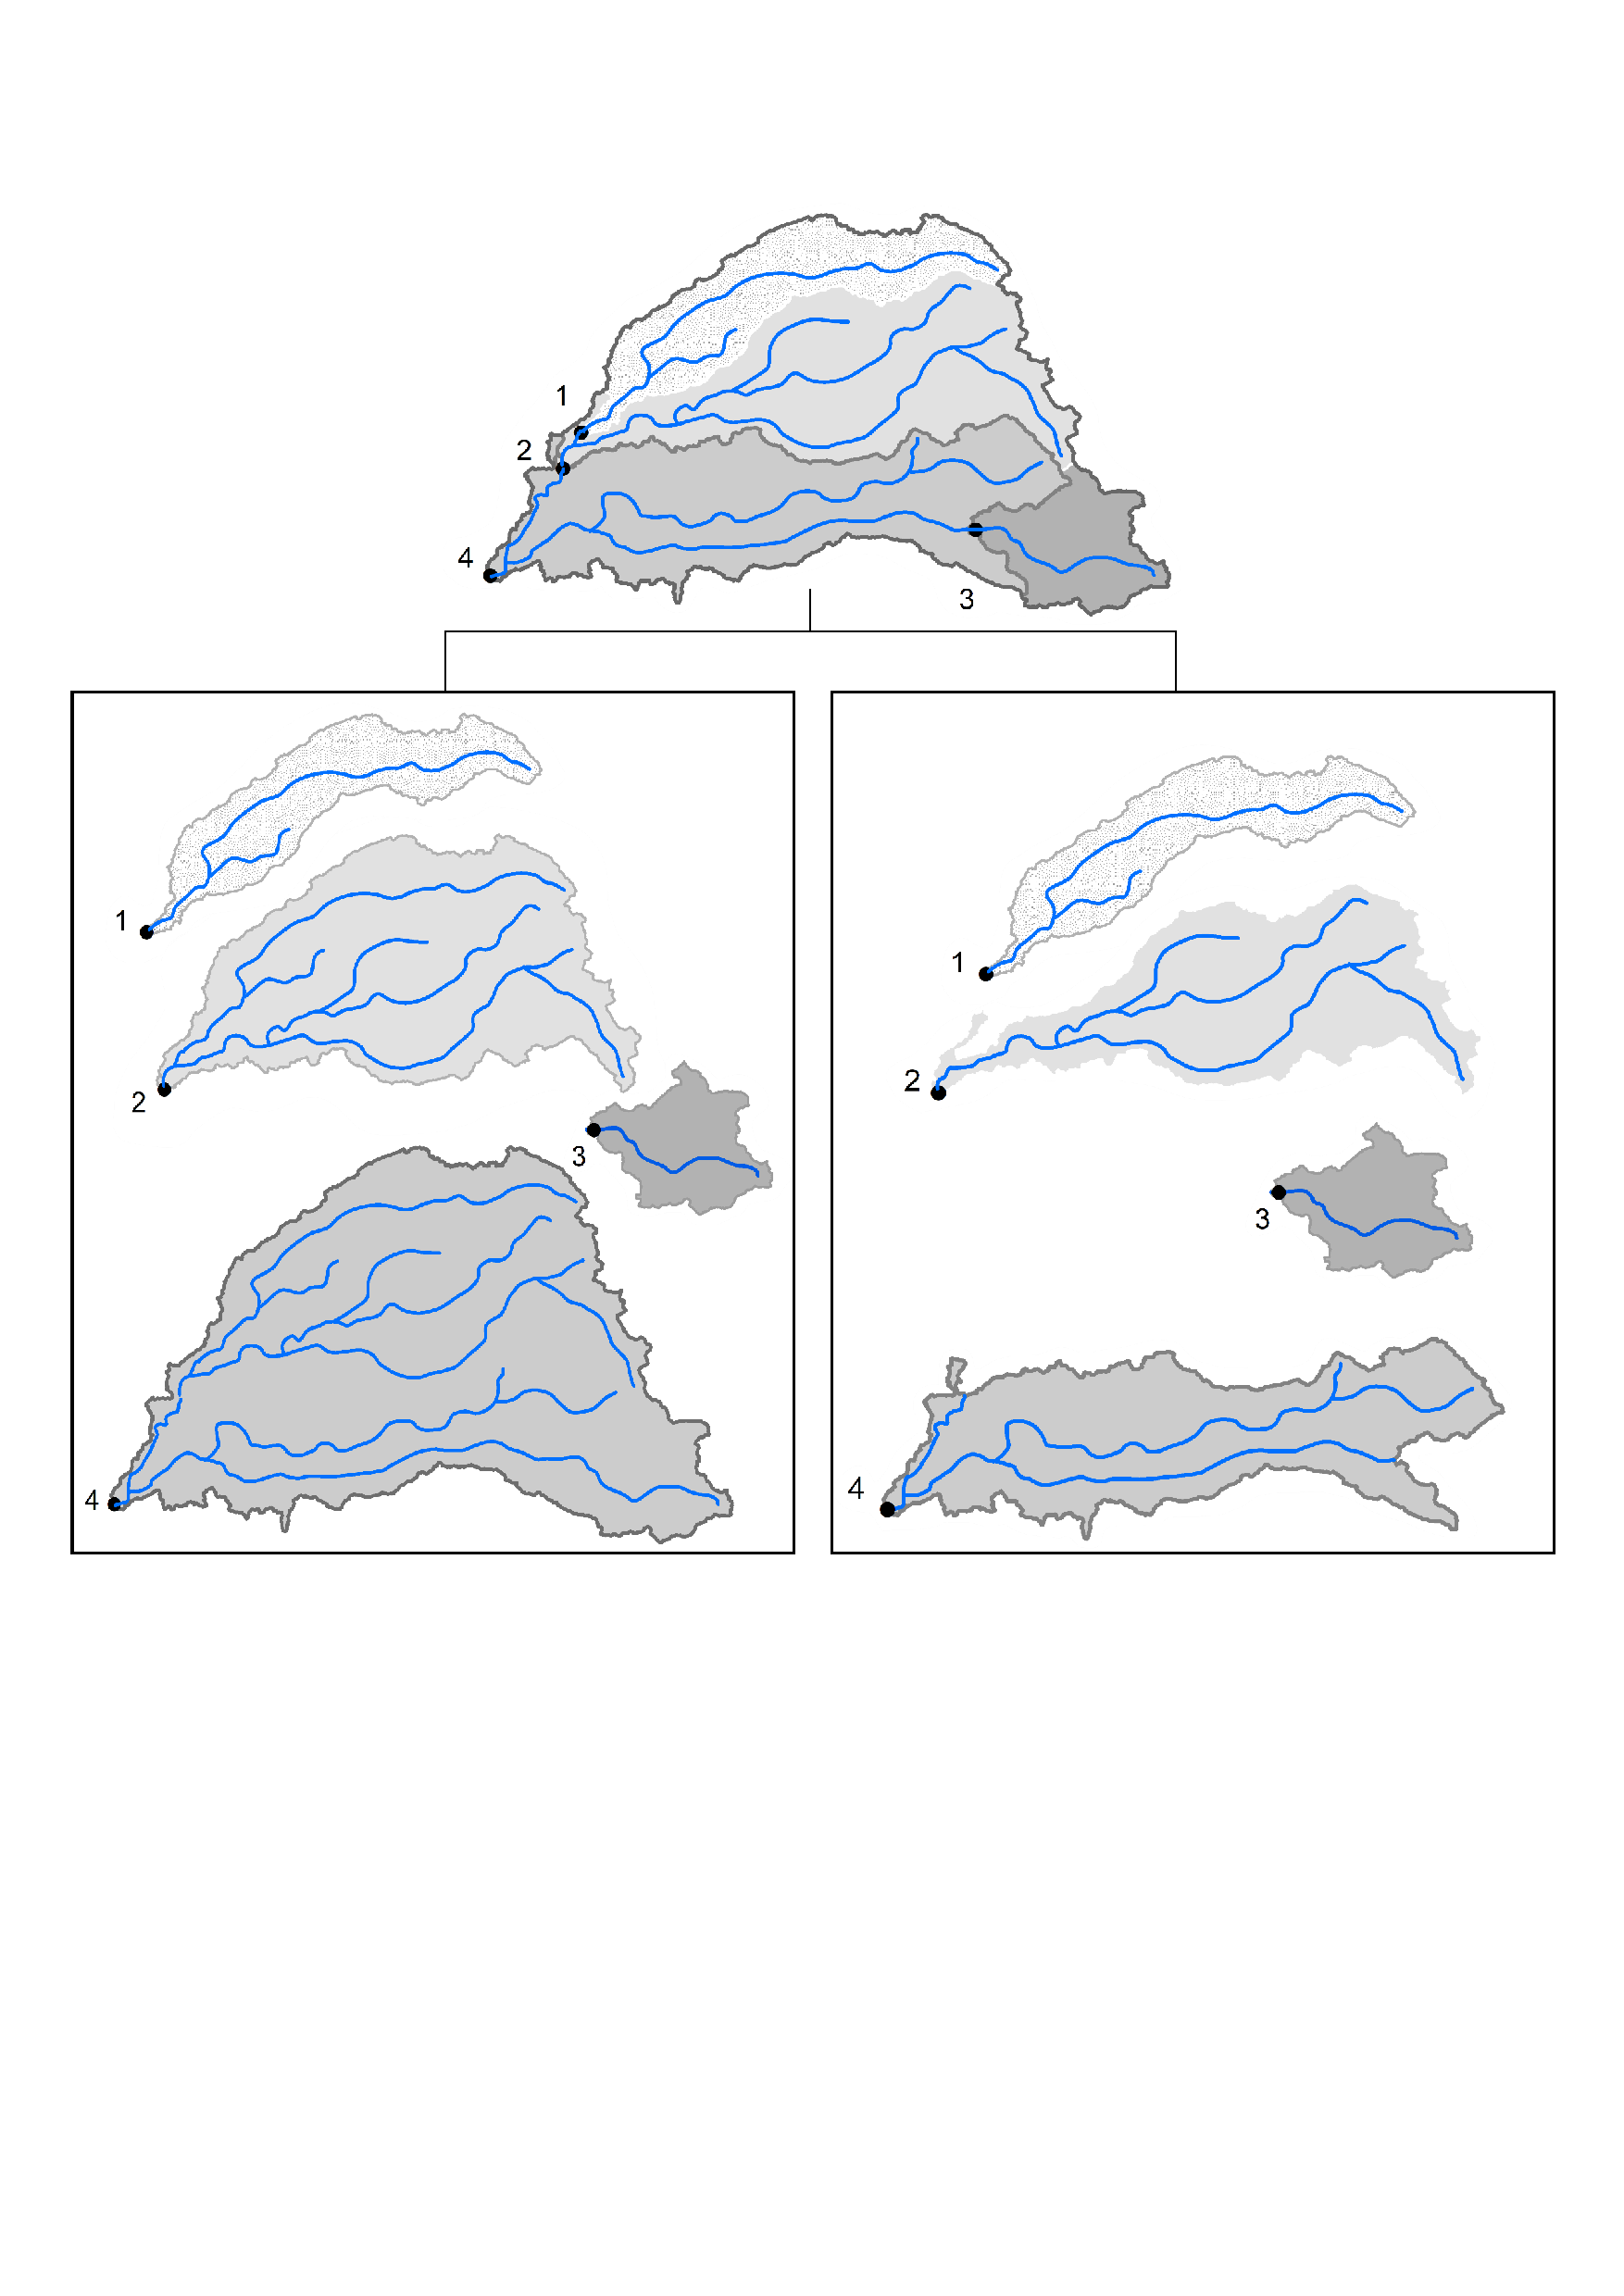
\includegraphics[width=\textwidth, trim={0 29.5cm 0 3.8cm}, clip=true]{plots/agg_and_inc_basins.pdf}
	\end{subfigure}% 
	\hfill
	\begin{subfigure}{.35\textwidth}
  		\centering
 		 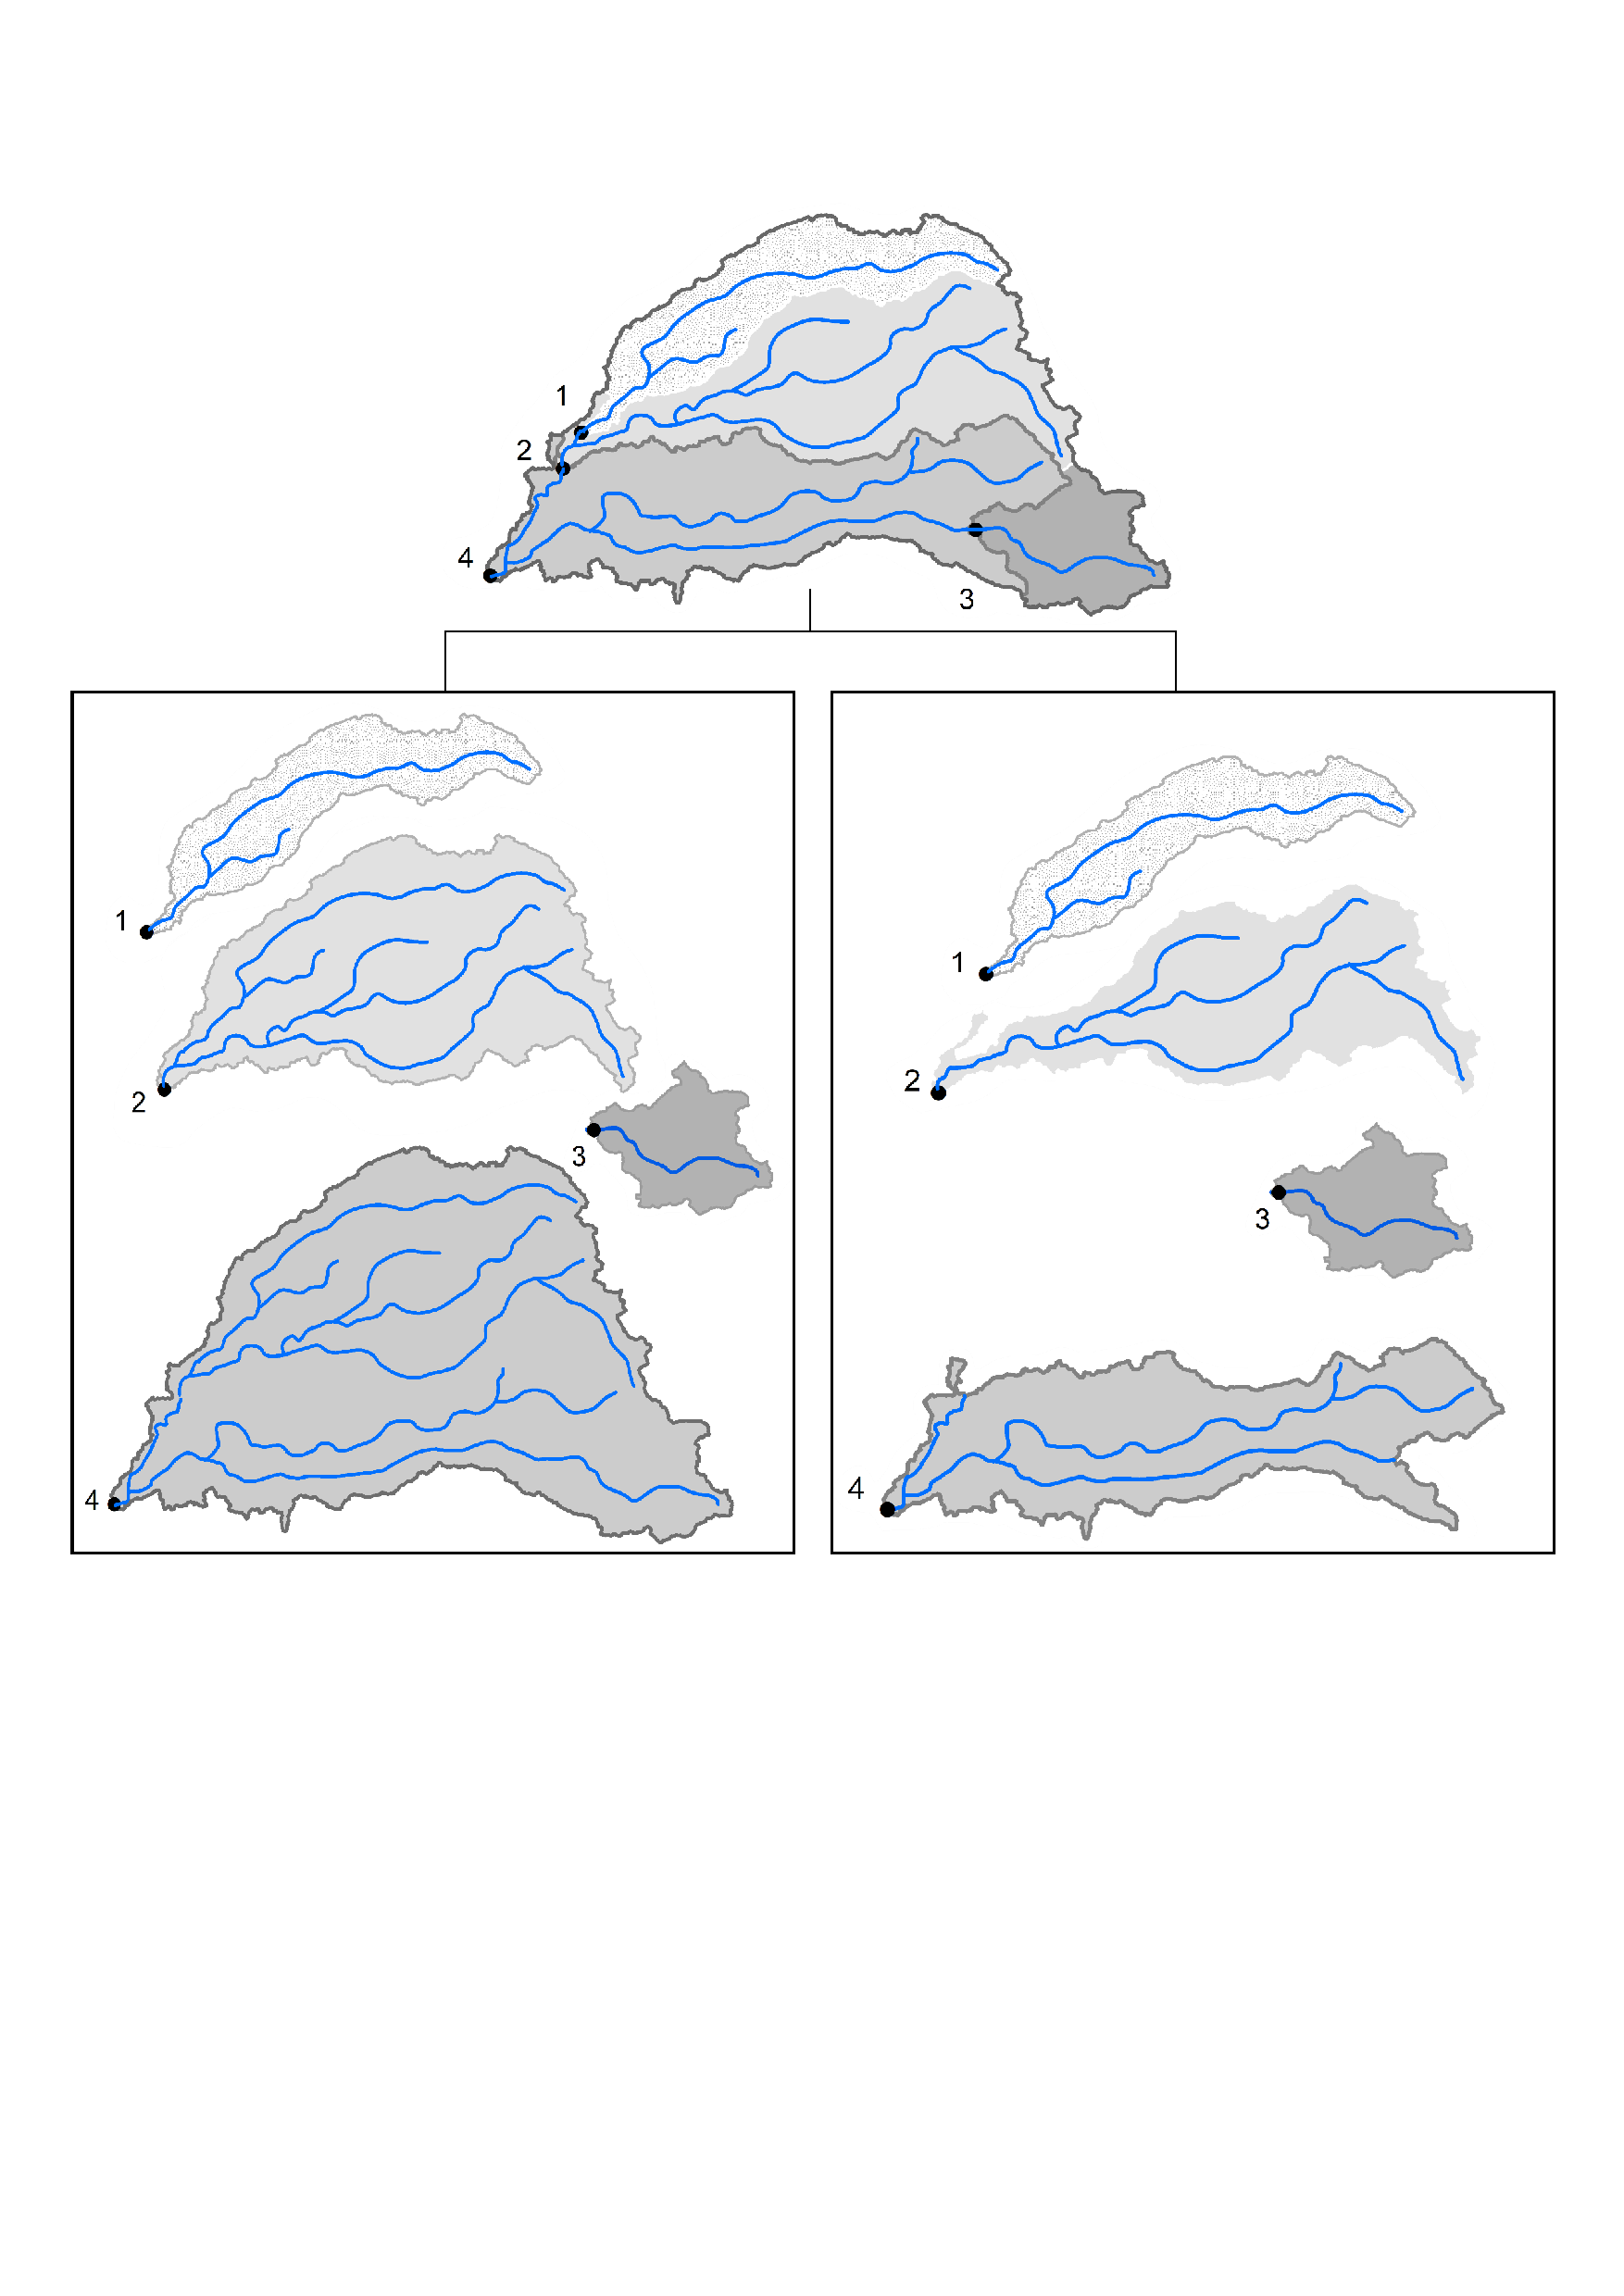
\includegraphics[width=\textwidth, trim={0 13cm 15cm 12.65cm}, clip=true]{plots/agg_and_inc_basins.pdf}
  		\caption{Aggregate Basins}
  		\label{fig:aggbasins}
	\end{subfigure}% 
	\begin{subfigure}{.35\textwidth}
  		\centering
  		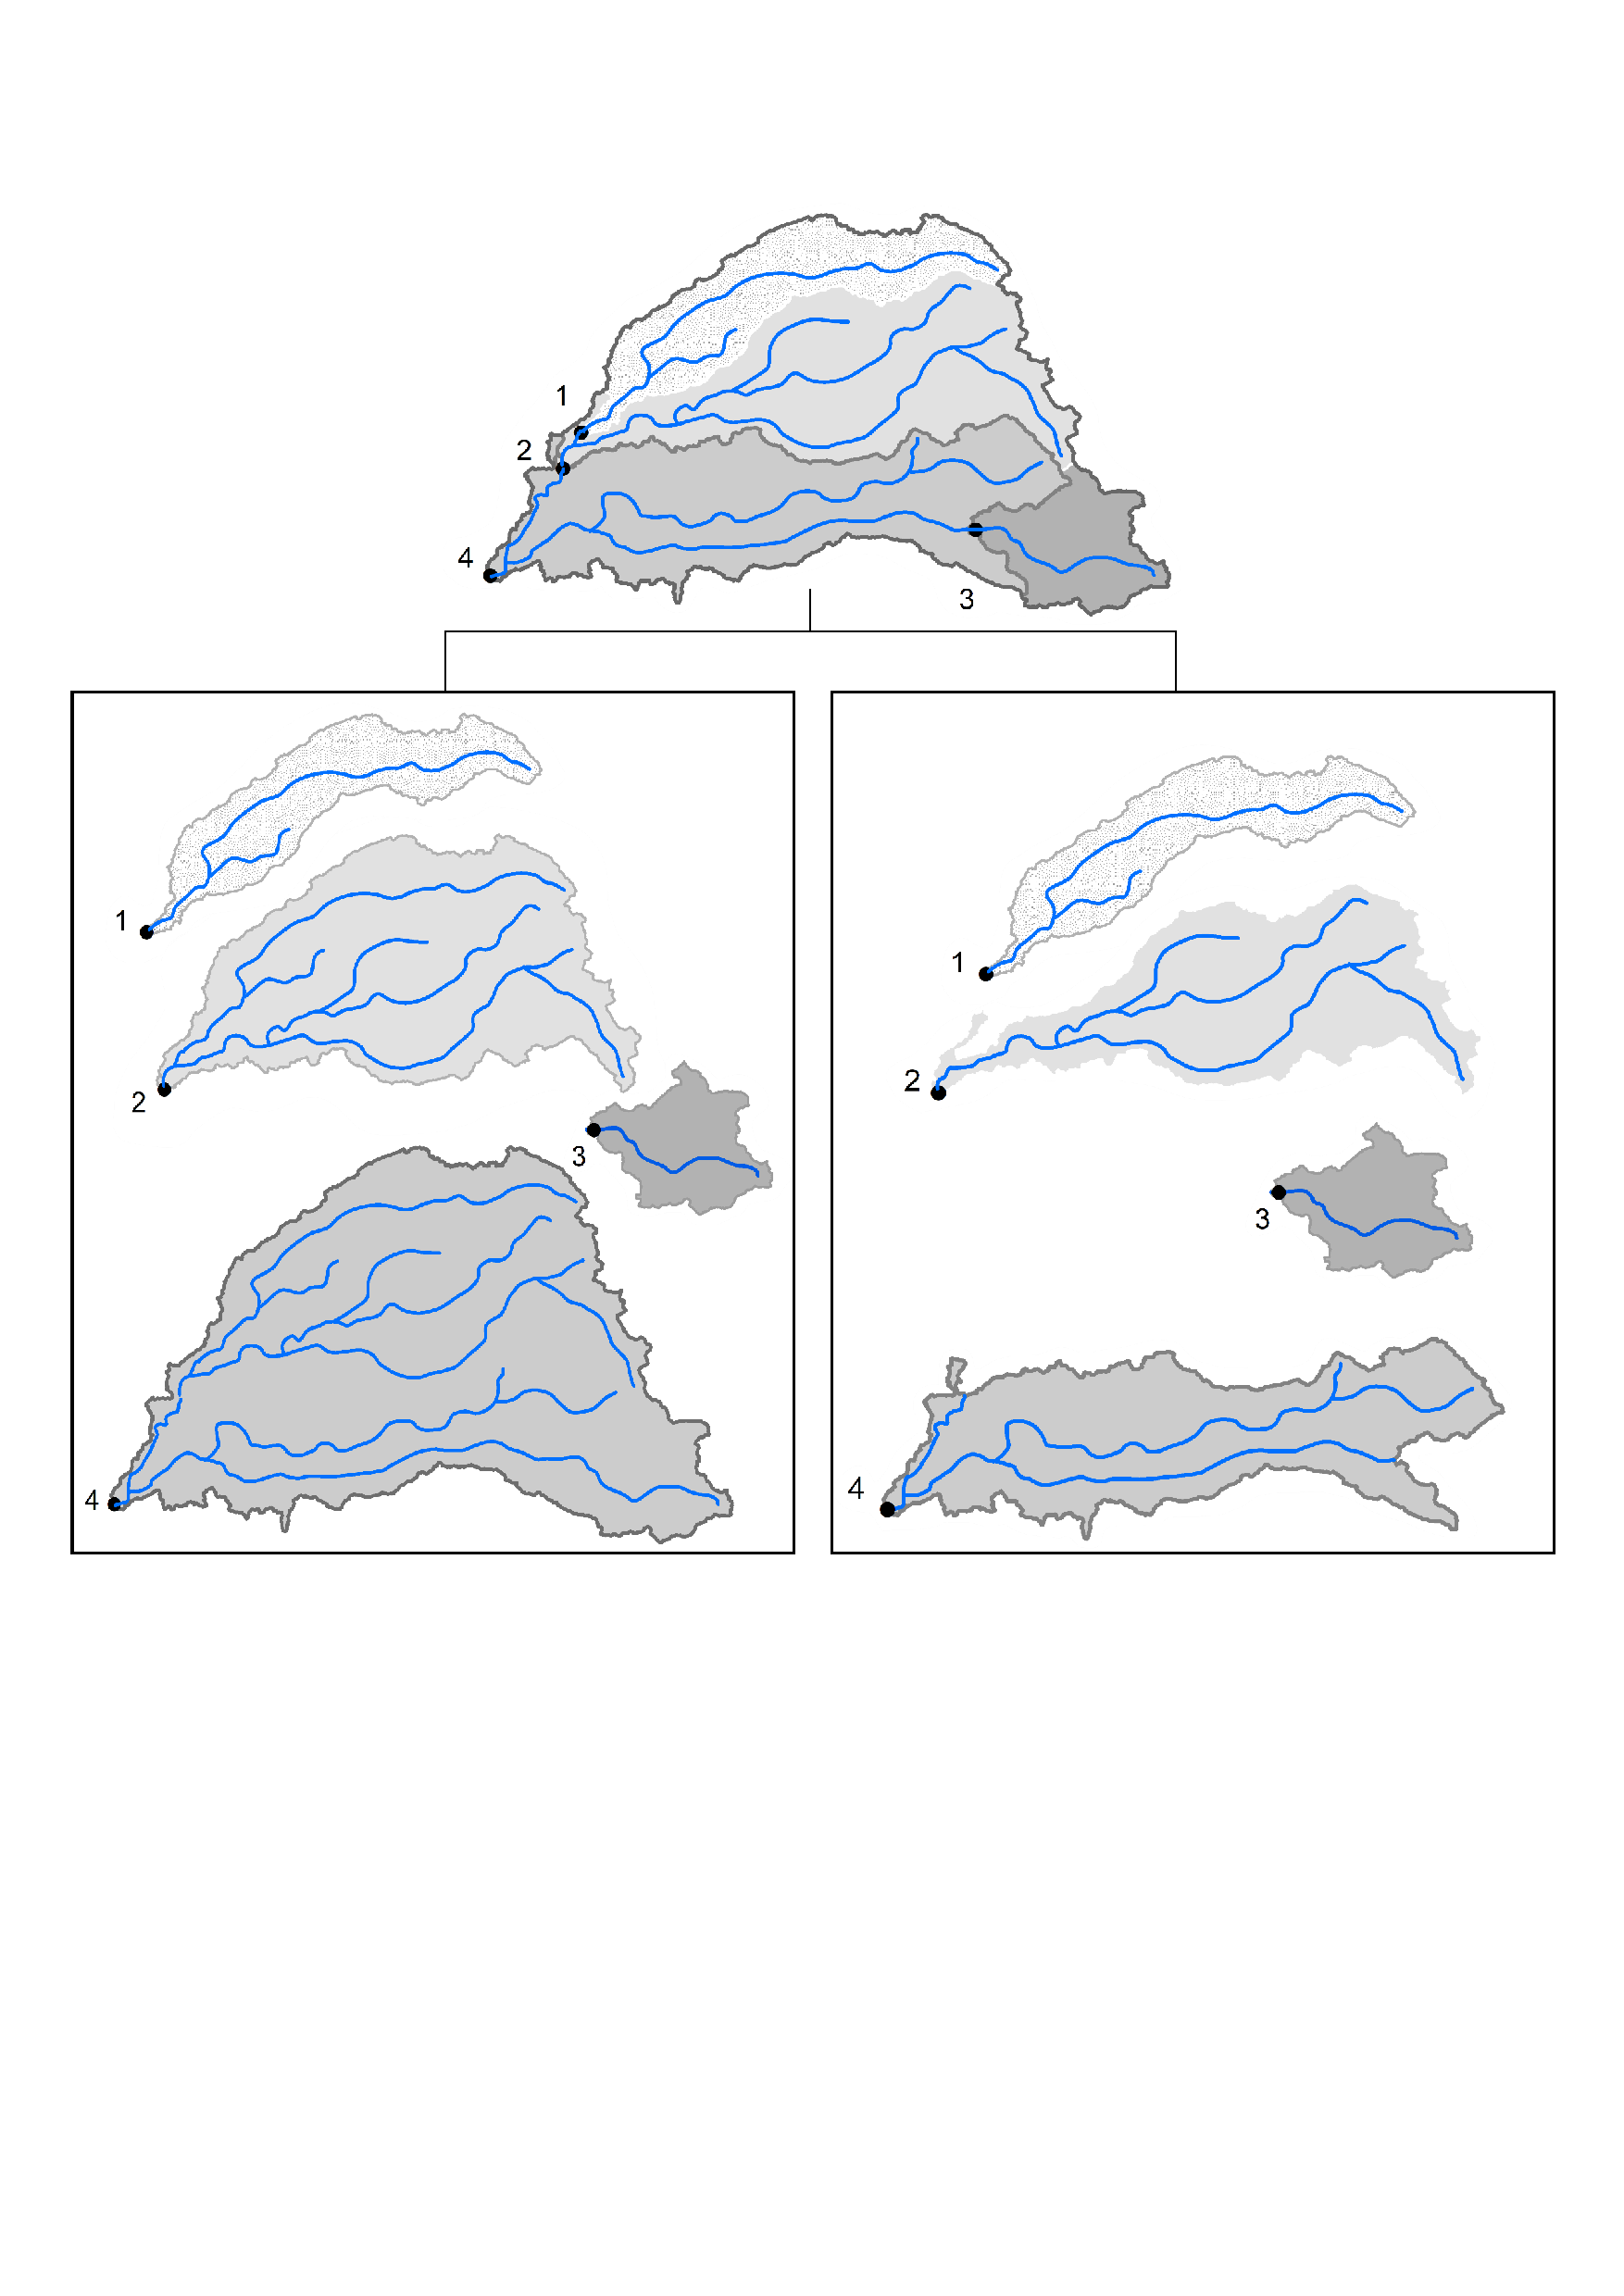
\includegraphics[width=\textwidth, trim={15cm 13cm 0 12.65cm}, clip=true]{plots/agg_and_inc_basins.pdf}
  		\caption{Incremental Basins}
  		\label{fig:incbasins}
	\end{subfigure}
	\caption{A basin's hydrologic response can be interpreted in two fundamentally different ways: (a) aggregate basins, where each basin's response is a function of all the land above the outlet that drains to the outlet, or (b) incremental basins, where each piece of land below an outlet incrementally alters the observed flows from gauges above it.}
	\label{fig:aggincbasins}
\end{figure}

% In addition, the unimpaired flows can be presented in a cumulative form, starting with zero at the beginning of the \textit{water year}. Water years are different from normal calendar years, since part of the precipitation that falls in late fall and winter accumulates as snow and does not drain until the following spring or summer's snowmelt. In California, each year's water year starts on the October of the year before. Hydrologists, sometimes, model and use the cumulative form of precipitation and runoff rather than their non-cumulative values. 

In this chapter, we have two types of data pre-processing: aggregate and incremental basins. Each data transformation method reflects our way of viewing hydrologic processes. Neither is ``right" as they are merely philosophical views of hydrologic processes. 

%----------------------------------------------------------------------------------------------------------------------------------------------------------------------------------------------------------
\section{Methods}
%-----------------------------------------------
\subsection{Model Types and Loss Functions}
The models considered and their parameters are explained below (Table \ref{table:modelspar}).

\begin{table*}[h]\renewcommand{\arraystretch}{1} 
	\linespread{1.0}
	\centering
	\caption{Model types and their parameters.}
	\begin{tabular}{p{1.5cm}p{2.5cm}p{5.5cm}p{5cm}} % must add to 16.5
		\toprule
		Model & R & Parameters defined in  & Parameters selected\\
		type & package & model formulation & through cross validation\\
		\midrule
		LM & stats & not applicable & not applicable\\
		\addlinespace
		GLM & stats & family=Tweedie & var.power=1.1 \\
		& statmod & link.power=0 & \\
		& & maxit=1000 & \\
		\addlinespace
		RF & randomForest & ntree=500 & mtry=20\\
 		&  & sampsize=length(training set) & \\
 		&  & nodesize=5 & \\
		\addlinespace
		NN & keras & batch\_size=25 & epochs=100 \\
 		&  & validation\_split=0.2 & \\
		\bottomrule
	\end{tabular}
	\label{table:modelspar}
\end{table*}

%-----------------------------------------------
\subsubsection*{Linear Multivariate Regression Models}
In 1805, Adrien Marie Legendre introduced the least squares method of estimating parameters as an appendix to his book on the paths of comets. A few years later, Carl Freidrich Gauss also published the method \cite{stigler1981gauss}. The method is brought to perfection with its application to linear regression and curve fitting. 

Linear Multivariate Regression models (LM) are customarily made of systematic and random error components, where the errors are usually assumed to have Normal distribution (Equation \ref{eq:lmdef}). 
\begin{equation} \label{eq:lmdef}
	\begin{aligned}
		& Y \sim N(\mu, \sigma \textsuperscript{2}) \mathrm{: random}  \\
		& \mu=X\beta \mathrm{: systematic}
	\end{aligned}
\end{equation} 

Given the model, the fitted values can be estimated by Equation \ref{eq:fitted}.
\begin{equation} \label{eq:fitted}
	Y^{sim}_i = \beta_{0} +\beta_{1} X_{1i} +\beta_{2} X_{2i} +\cdots +\beta_{i} X_{ki}
\end{equation} 

The unknown parameters in Equation \ref{eq:fitted} are: $\beta_{0}$ (the overall mean) and $\beta_{k}$ (the regression coefficients). To find the best fit, much like simple linear regression, we need to estimate the unknown parameters by minimizing a loss function, customarily the residual sum of squares (RSS) (Equation \ref{eq:rss}).

\begin{equation} \label{eq:rss}
	\begin{split}
		RSS &= \sum^n_{i=1}e^{2}_{i} \\
		&= \sum^n_{i=1}(Y^{obs}_{i} - y^{sim}_i)^2 \\
		&= \sum^n_{i=1}(Y^{obs}_{i}-\beta_{0} +\beta_{1} X_{1i} +\beta_{2} X_{2i} +\cdots +\beta_{i} X_{ki})
	\end{split}
\end{equation} 

The {\tt lm()} function in R constructs LMs. They are easy to understand and interpret, which makes them a great first cut at predictive modeling. However, they over simplify reality (hydrologic processes are not linear) and lack precision (as demonstrated by the goodness-of-fit measures). Another major flaw is that a linear predictor can give predictions that are physically impossible (e.g., negative flows). Here, the variance cannot be considered constant since there is a boundary on the response. These shortcomings can be overcome with generalized linear models. 

%-----------------------------------------------
\subsubsection*{Generalized Linear Regression Models}
In 1972, Nelder and Wedderburn introduced Generalized Linear Regression models \linebreak (GLM). This work allowed for a unified fitting procedure, despite the type of error distribution, based on likelihood \cite{nelder1972generalized}. Therefore, unlike LMs, GLMs can accommodate non-Normal distributions of error. However, except for Normal distributions most other distributions do not have a closed-form solution. 

In GLMs, the linear model is related to the response variable via a link function. This function allows the magnitude of the variance of each measurement to be a function of its predicted value. Therefore a GLMs components are (Equation \ref{eq:glmdef}): 
\begin{equation} \label{eq:glmdef}
	\begin{aligned}
		& Y \sim P(\mu, \phi)  \mathrm{: random}\\
		& g(\mu)=X\beta \mathrm{: systematic}
	\end{aligned}
\end{equation} 

Where P is the distribution of random errors, and $g(\mu)$ is the link function. P and g can be specified by the user.

The {\tt glm()} function in R constructs GLMs. The GLMs developed here are characterized by the \textit{Tweedie distribution}, since the outcome (i.e., unimpaired flow) is continuous, non-negative, skewed, and unbalanced with exact zeros. Tweedie distributions are a special case of exponential dispersion models where the variance function is a power function (Equation \ref{eq:glmvar}), and the link, or the function used to explain how the expectation of the outcome is related to the linear predictor can be specified in terms of Box-Cox transformations \cite{jorgensen1997theory}.
\begin{equation} \label{eq:glmvar}
	var(Y)=V(\mu)\phi=\mu^\alpha \phi
\end{equation}

The power, alpha, can be set by the user, or determined through cross-validation. Special cases include Normal ($\alpha$=0), Poisson ($\alpha$=1), Gamma ($\alpha$=2), and inverse-Gaussian ($\alpha$=3) GLMs . Here, we set the power $\alpha$ to be 1.1. The link $g$ can be specified as log or identity. Here, we used the log link. 

Therefore, the above model assumes that $y_i \sim Tweedie_{\alpha}(\mu_i, \phi)$ where
\begin{equation*}
	var(Y_i)=\mu_i^{1.1} \phi
\end{equation*}
and 
\begin{equation*}
	log(\mu_i)=\beta_{0} +\beta_{1} X_{1i} +\beta_{2} X_{2i} +\cdots +\beta_{i} X_{ki}
\end{equation*}

The regression coefficients, $\beta_{j}$, were estimated by maximum likelihood. The dispersion parameter, $\phi$, was estimated using the residual sum of squared residuals, otherwise called the Pearson estimator.

Both LMs and GLMs are parametric models. For prediction purposes non-parametric methods are proven to perform better since their form is shaped by the data and not fixed a priori. Therefore, next, we consider a non-parametric modeling method, random forests. 

%-----------------------------------------------
\subsubsection*{Tree Building Algorithms} 
Classification and Regression Trees (CARTs) involve stratifying or segmenting the predictor space, into a number of regions, using a series of if-then statements. At each internal node in the tree, a test is made to one of the inputs. Depending on the outcome of the test (or split rule), the algorithm goes to either the left or the right sub-branch of the tree. Eventually the algorithm arrives at a terminal node, which contains a prediction. The prediction for a given observation is the mean or the mode of the training observations in the region to which it belongs \cite{breiman1984classification}. 

 In essence, each tree is a series of split rules. The split rule is found using a greedy top-down search for recursively splitting of the data into binary partitions. It is greedy, because, the split rule at each internal node is selected to maximize the homogeneity of its child nodes, without consideration of nodes further down the tree, yielding only locally optimal trees \cite{grubinger2011evtree}. For regression trees, the mean of all the observation points that fall within a branch is considered the prediction of that branch in the tree. The best tree is one which has the minimum test error rate calculated by the RSS. 

Since trees have a finite number of terminal nodes (CARTs are pruned based on a complexity parameter, $\alpha$), the prediction of these methods are discrete, and therefore, not particularly suited to modeling a continuous variable. In addition, CARTs suffer from high variance; trees grown on different subsets of the training set will produce different predictions. This phenomenon is one of the major drawbacks of CARTs. Methods such as \textit{bagging} \cite{breiman1996bagging}, \textit{random forests} \cite{breiman2001random}, \textit{boosting} \cite{friedman2001greedy} and \textit{bumping} \cite{grubinger2010regression} attempt to improve the prediction accuracy of trees with the idea that combining and averaging trees reduces variance. 

A Random Forest (RF) consists of an assemblage of unpruned CART models. Each CART model in an RF is different because it is grown using: (1) a new training set: in each bootstrapped training set, about one-third of the instances are left out; and (2) random feature selection: each time a split in a tree is considered, a random sample of predictors is chosen as split candidates from the full set of predictors. This process de-correlates the trees. 
%Suppose there is one very strong predictor in the dataset, along with other moderately strong predictors. Then, in the collection of trees, most or all trees will use this strong predictor in the top split. Consequently, all trees will look quite similar. So, the predictions from the trees will be highly correlated. However, by forcing each split to consider only a subset of the predictors makes the resulting trees less variable and more reliable \cite{james2013introduction}. 
This strategy, using a random selection of features to split each node, introduces some randomness that improves the accuracy of the predictions of the trees as a whole and yields error rates that are robust with respect to noise \cite{breiman2001random}.

%\begin{equation} \label{eq:rfdef}
%	\hat {y} = {\frac {1}{m}}\sum _{j=1}^{m}\sum _{i=1}^{n}W_{j}(x_{i},x')\,y_{i}=\sum _{i=1}^{n}\left({\frac {1}{m}}\sum _{j=1}^{m}W_{j}(x_{i},x')\right)\,y_{i}
%\end{equation}
%
%Equation \ref{eq:rfdef} shows that the RF is essentially a weighted neighborhood scheme, with weights that average of the individual trees.

The {\tt randomForest()} function in the {\tt randomForest} library \cite{liaw2002classification}, constructs RF models. This function takes in tuning parameters such as mtry, ntree, sampsize, and maxnodes:

{\tt mtry}: In RFs, internal estimates monitor error, strength and correlation, which are used to show the response to increasing the number of features used in the splitting. Here, this parameter was set to 20 out of the full 25 predictor variables available found through cross-validation.

{\tt ntree}: The generalization error of a forest of trees depends on the strength of the individual trees in the forest and the correlation between them \cite{breiman2001random}. This error converges to a limit as the number of trees in the forest increases. Here, the number of trees was set to the default 500. 

{\tt sampsize}: In RFs, the trees are built on a bootstrap sample of the training data, a sample equal in size to the original dataset, but selected with replacement. Therefore, some observations are not selected, and others are selected more than once. Here, the sample size is set to the default value, the length of the training set.

{\tt maxnodes}: Using the maximum number of terminal nodes, the user can ``prune'' the trees back to a smaller version of itself. Here, we used the default value, which is a function of {\tt nodesize} or the allowed minimum number of observations in each node. The default value for nodesize is 5.   

% These parameters can be fixed by the user or optimized. The benefit of optimizing the parameters become evident when overfitting is concerned \cite{breiman2001random}. Figure \ref{fig:optsettings} shows that, with the exception of mtry, the optimal parameters are the default parameters for this study. 

Like LMs, RFs also typically use the RSS loss function to find the optimal split value. For more information about loss functions see Chapter \ref{ch3:loss}.

% In conclusion, the choice of a suitable model relies on striking the desired balance between three model properties: generality, reality, and precision. Therefore, model selection shouldn't solely rely on statistics; some models better reflect physical foundations in hydrology, and conceptual considerations need to include the desired level of trade-off between optimizing accuracy versus optimizing generality \cite{guisan2000predictive}. Unfortunately, no guide to empirical model selection exists in hydrology. 

%-----------------------------------------------
\subsubsection*{Neural Networks} 
In 1951, Marvin Minsky and graduate student Dean Edmonds built the first neural network (NN) machine. This machine was a randomly connected network of capacitors that have a finite amount of memory and time to keep or remember that memory. The memory holds the probability that a signal will come in one input and another signal will come out of the output. This machine, modeled after the Hebbian theory of learning in the human brain, was one of the first pioneering attempts at artificial intelligence. Shortly after, in 1957, Frank Rosenblatt invents the perceptron, the first \textbf{neural network} for computers. 

[INSERT neural network graph, equation, chain rule for finding optimal parameters, insert discussion on model variables and their specifications] 

%-----------------------------------------------
\subsection{Test Error Approximation}
Blocking cross-validation is used to approximate the test set error. Here, all data for the basin to be modeled is left out of the training data and becomes the test set (i.e., leave one group out cross validation). Therefore, the training data is the data from all the other basins. This process was repeated for all basins in the study, and so, for model evaluation, one LM, GLM, RF, and NN model exists for each basin. For more information about resampling methods see Chapter \ref{ch4:resampling}.

With the developed model's predictions and the observations in the test set, we can calculate the desired model goodness-of-fit: Bias-Corrected Coefficient of Determination (bR\textsuperscript{2}) and Nash-Sutcliffe Efficiency factor (NSE) (Equations \ref{eq2:r2}, \ref{eq2:br2}, and  \ref{eq2:nse}). See appendix \ref{d:mof} for more model measures-of-fit.

\begin{equation} \label{eq2:r2}
	R^{2} = \ \left(\frac{\sum^n_{i=1}{\left(Y^{obs}_i-\overline{Y^{obs}}\right)\left(Y^{sim}_i-\overline{Y^{sim}}\right)}}{\sqrt{\sum^n_{i=1}{\left(Y^{obs}_i-\overline{Y^{obs}}\right)^2}}\sqrt{\sum^n_{i=1}{\left(Y^{sim}_i-\overline{Y^{sim}}\right)^2}}}\right)^2  \quad R^{2} \in [0,1] \\
\end{equation}

$R^2$ is insensitive to additive and proportional difference between model simulation and observations. One can simply show that for a non zero value of $\beta_0$ and $\beta_1$, if the predictions follow a linear form, $Y^{sim}=\beta_0 + \beta_1 Y^{obs}$, the $R^2$ equals one \cite{legates1999evaluating}. Therefore, for a proper model assessment, it is recommended that the slope of the predicted vs. observed graph be reported or systematically included as in Equation \ref{eq2:br2}. 

\begin{equation} \label{eq2:br2}   
	bR^{2} =  
	\begin{cases}
		\text{$\abs{b}R^2$} & \quad\text{for b}\le1\\
		\text{$\abs{b}^{-1}R^2$} &\quad\text{for b}>1  \quad bR^{2} \in [0,1] \\
	\end{cases}
\end{equation}

By weighting $R^2$, under and over predictions are quantified together with the model dynamics which results in a more comprehensive reflection of model results.

Another commonly used model goodness-of-fit is the the Nash-Sutcliffe efficiency factor (Equation \ref{eq:nse}). 

\begin{equation} \label{eq2:nse}
	NSE =\ 1-\frac{\sum^n_{i=1}{{\left(Y^{sim}_i-Y^{obs}_i\right)}^2\ }}{\sum^n_{i=1}{{\left(Y^{obs}_i-\overline{Y^{obs}}\right)}^2\ }} \quad NSE \in (-\infty,1] 
\end{equation}

A Nash-Sutcliffe efficiency factor of lower than zero indicates that the mean value of the observed time series would have been a better predictor than the model. Like the bR\textsuperscript{2}, the largest disadvantage of the Nash-Sutcliffe efficiency factor is the fact that the differences between the observed and predicted values are calculated as squared values. As a result, larger values in a time series are strongly overestimated whereas lower values are neglected \cite{legates1999evaluating}. For the quantification of runoff predictions this leads to an overestimation of the model performance during peak flows and an underestimation during low flow conditions \cite{krause2005comparison}.

%-----------------------------------------------
\subsection{Post-Processing}
In post-processing all model predictions are modified so as to be comparable to original gauge flows; all cumulative values are back-transformed into non-cumulative forms, and all incremental basins are back-transformed into aggregate forms. In other words, the steps used in pre-processing are reversed so as to fairly compare the goodness-of-fit across all models.

%------------------------------------------------------------------------------------------------------------------------------------------------------------------------
\section{Results}

%-----------------------------------------------
\subsection{Model Evaluation}
Figure \ref{fig:obsvpred} shows the predicted unimpaired flows versus the observed for each model type in order of increasing NSE. A perfect model will follow the $y=x$ line. The regression line shows a tendency for the LM and RF aggregate and incremental models to under predict and for the GLM aggregate and incremental models to slightly over predict the unimpaired flows. Under predicting flows are generally bad in times of floods and over predicting flows are generally bad in times of droughts, since both lead to decisions that are both inaccurate and not conservative. The NN outperforms other models and it is somewhat insensitive to the input data pre-processing.

% Squared error loss functions tend to predict large values at the expense of smaller ones, since larger errors have more of a penalty (i.e., are being squared). Hence, the models failure at modeling basins at a low hierarchy compared to higher hierarchies. This phenomenon will be explored in other chapters. 

%\begin{figure}
%	\centering
%	\begin{subfigure}{.5\textwidth}
%  		\centering
% 		 \includegraphics[width=\textwidth, trim={0 0 0 0}, clip=true]{plots/rplot27_obsvspred2_lm_agg.png}
%  		\caption{LM Aggregate}
%  		\label{fig:lmagg}
%	\end{subfigure}% 
%	\begin{subfigure}{.5\textwidth}
%  		\centering
% 		 \includegraphics[width=\textwidth, trim={0 0 0 0}, clip=true]{plots/rplot27_obsvspred2_lm_inc.png}
%  		\caption{LM Incremental}
%  		\label{fig:lminc}
%	\end{subfigure}% 
%	\hfill
%	\begin{subfigure}{.5\textwidth}
%  		\centering
% 		 \includegraphics[width=\textwidth, trim={0 0 0 0}, clip=true]{plots/rplot27_obsvspred2_glm_agg.png}
%  		\caption{GLM Aggregate}
%  		\label{fig:glmagg}
%	\end{subfigure}% 
%	\begin{subfigure}{.5\textwidth}
%  		\centering
% 		 \includegraphics[width=\textwidth, trim={0 0 0 0}, clip=true]{plots/rplot27_obsvspred2_glm_inc.png}
%  		\caption{GLM Incremental}
%  		\label{fig:glminc}
%	\end{subfigure}% 
%	\hfill
%	\begin{subfigure}{.5\textwidth}
%  		\centering
% 		 \includegraphics[width=\textwidth, trim={0 0 0 0}, clip=true]{plots/rplot27_obsvspred2_rf_agg.png}
%  		\caption{RF Aggregate}
%  		\label{fig:rfagg}
%	\end{subfigure}% 
%	\begin{subfigure}{.5\textwidth}
%  		\centering
% 		 \includegraphics[width=\textwidth, trim={0 0 0 0}, clip=true]{plots/rplot27_obsvspred2_rf_inc.png}
%  		\caption{RF Incremental}
%  		\label{fig:rfinc}
%	\end{subfigure}% 
%	\hfill
%	\begin{subfigure}{.5\textwidth}
%  		\centering
% 		 \includegraphics[width=\textwidth, trim={0 0 0 0}, clip=true]{plots/rplot27_obsvspred2_nn_agg.png}
%  		\caption{NN Aggregate}
%  		\label{fig:nnagg}
%	\end{subfigure}% 
%	\begin{subfigure}{.5\textwidth}
%  		\centering
% 		 \includegraphics[width=\textwidth, trim={0 0 0 0}, clip=true]{plots/rplot27_obsvspred2_nn_inc.png}
%  		\caption{NN Incremental}
%  		\label{fig:nninc}
%	\end{subfigure}% 
%	\hfill
%	\caption{The models trained on the four types of data (i.e., aggregate, incremental, cumulative aggregate, and cumulative incremental). The LM generally underpredict unimpaired flows and show a bad fit. The GLMs slightly overpredict unimpaired flows, but show a better fit. The RF generally overpredict unimpaired flows. The RFs, non-parametric models, are a big improvement compared to the linear models, parametric models. Lastly, the NNs, out perform all models.}
%	\label{fig:obsvpred}
%\end{figure}

\begin{figure}
  	\centering
 	\includegraphics[width=\textwidth, trim={0 0 0 0}, clip=true]{plots/rplot27_obsvspred_all.png}
	\caption{The models trained on the four types of data (i.e., aggregate, incremental, cumulative aggregate, and cumulative incremental). The LM generally under predict unimpaired flows and show a bad fit. The GLMs slightly over predict unimpaired flows, but show a better fit. The RF generally over predict unimpaired flows. The RFs, non-parametric models, are a big improvement compared to the linear models, parametric models. Lastly, the NNs, out perform all models.}
	\label{fig:obsvpred}
\end{figure}

Figure \ref{fig:gof} shows how each model scores as to the bR\textsuperscript{2} and NSE. In the LM and GLM the incremental modeling method performs better than the aggregate. In the RF and NN their performances are very similar.

\begin{figure}
	\centering
	\begin{subfigure}{\textwidth}
  		\centering
 		 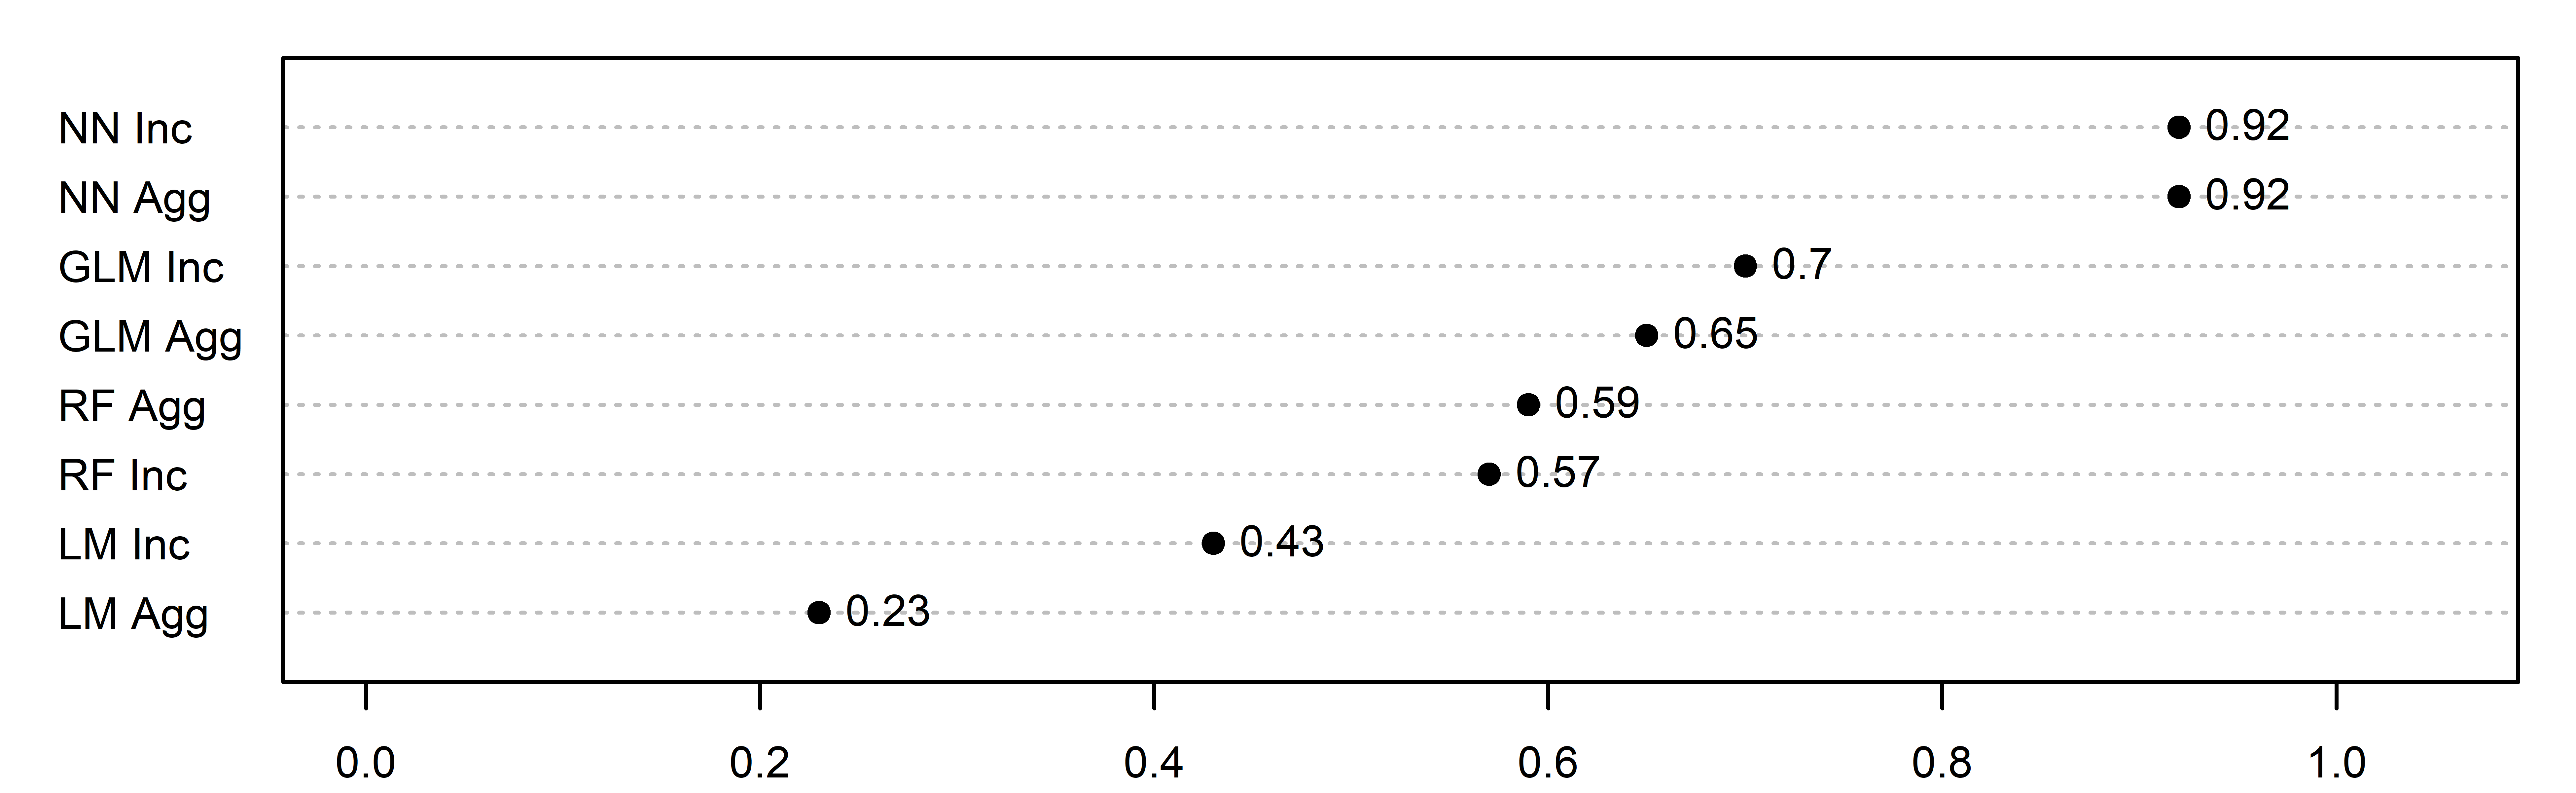
\includegraphics[width=\textwidth, trim={0 0 0 0}, clip=true]{plots/rplot26_gof_bR2.png}
  		\caption{bR\textsuperscript{2}}
  		\label{fig:rmse}
	\end{subfigure}%
	\hfill
	\begin{subfigure}{\textwidth}
  		\centering
  		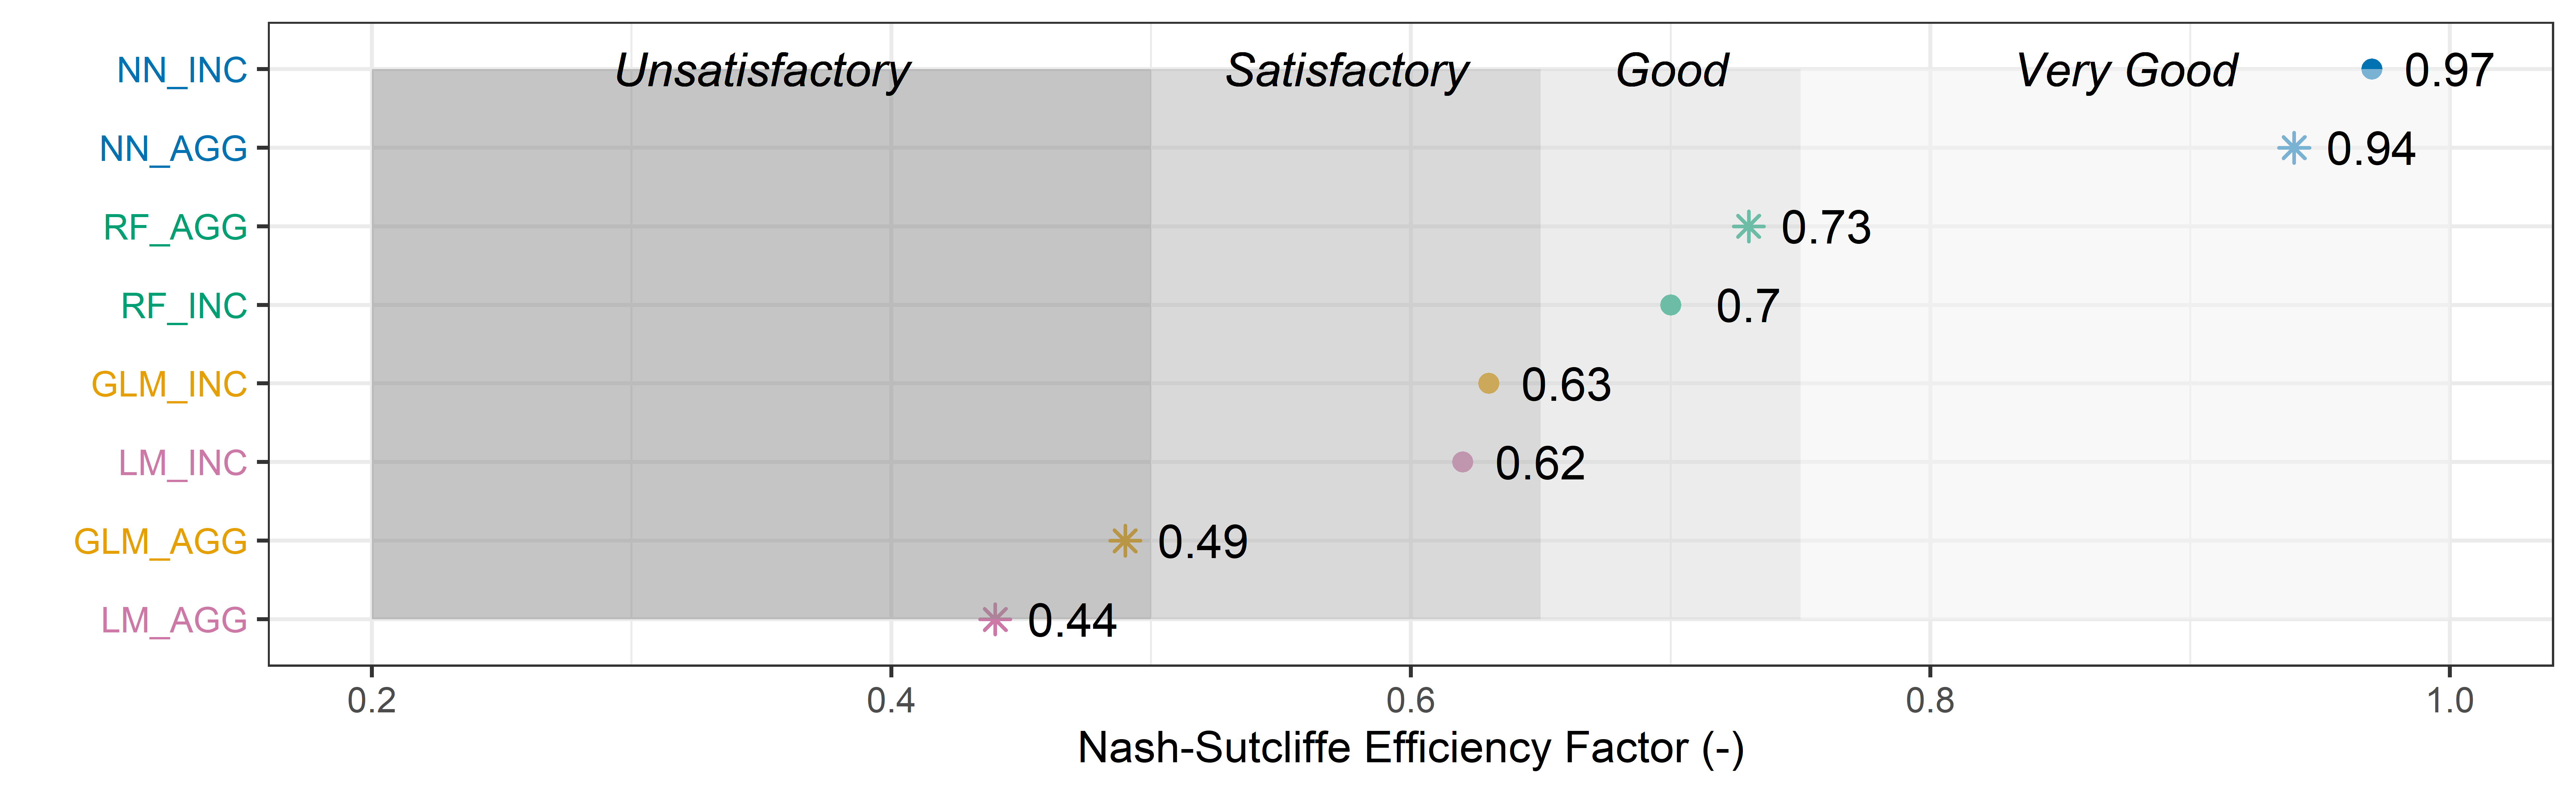
\includegraphics[width=\textwidth, trim={0 0 0 0}, clip=true]{plots/rplot26_gof_NSE.png}
  		\caption{NSE}
  		\label{fig:nse}
	\end{subfigure}
	\caption{The goodness-of-fit of models trained on the two types of data (i.e., aggregate and incremental) as measured by the Coefficient-of-Determination (bR\textsuperscript{2}) and Nash-Sutcliffe Efficiency (NSE). The NN aggregate and incremental model provides the best model performance in the bR\textsuperscript{2} and NSE respectively.}
	\label{fig:gof}
\end{figure}

Figure \ref{fig:resovertime} shows that the models all decrease in accuracy over time. We can hypothesize that this is due to climate change imposing non-stationarity on the hydrologic process. This is further discussed in chapter \ref{ch5:climatechange}.

\begin{figure}
	\centering
	\begin{subfigure}{.5\textwidth}
  		\centering
 		 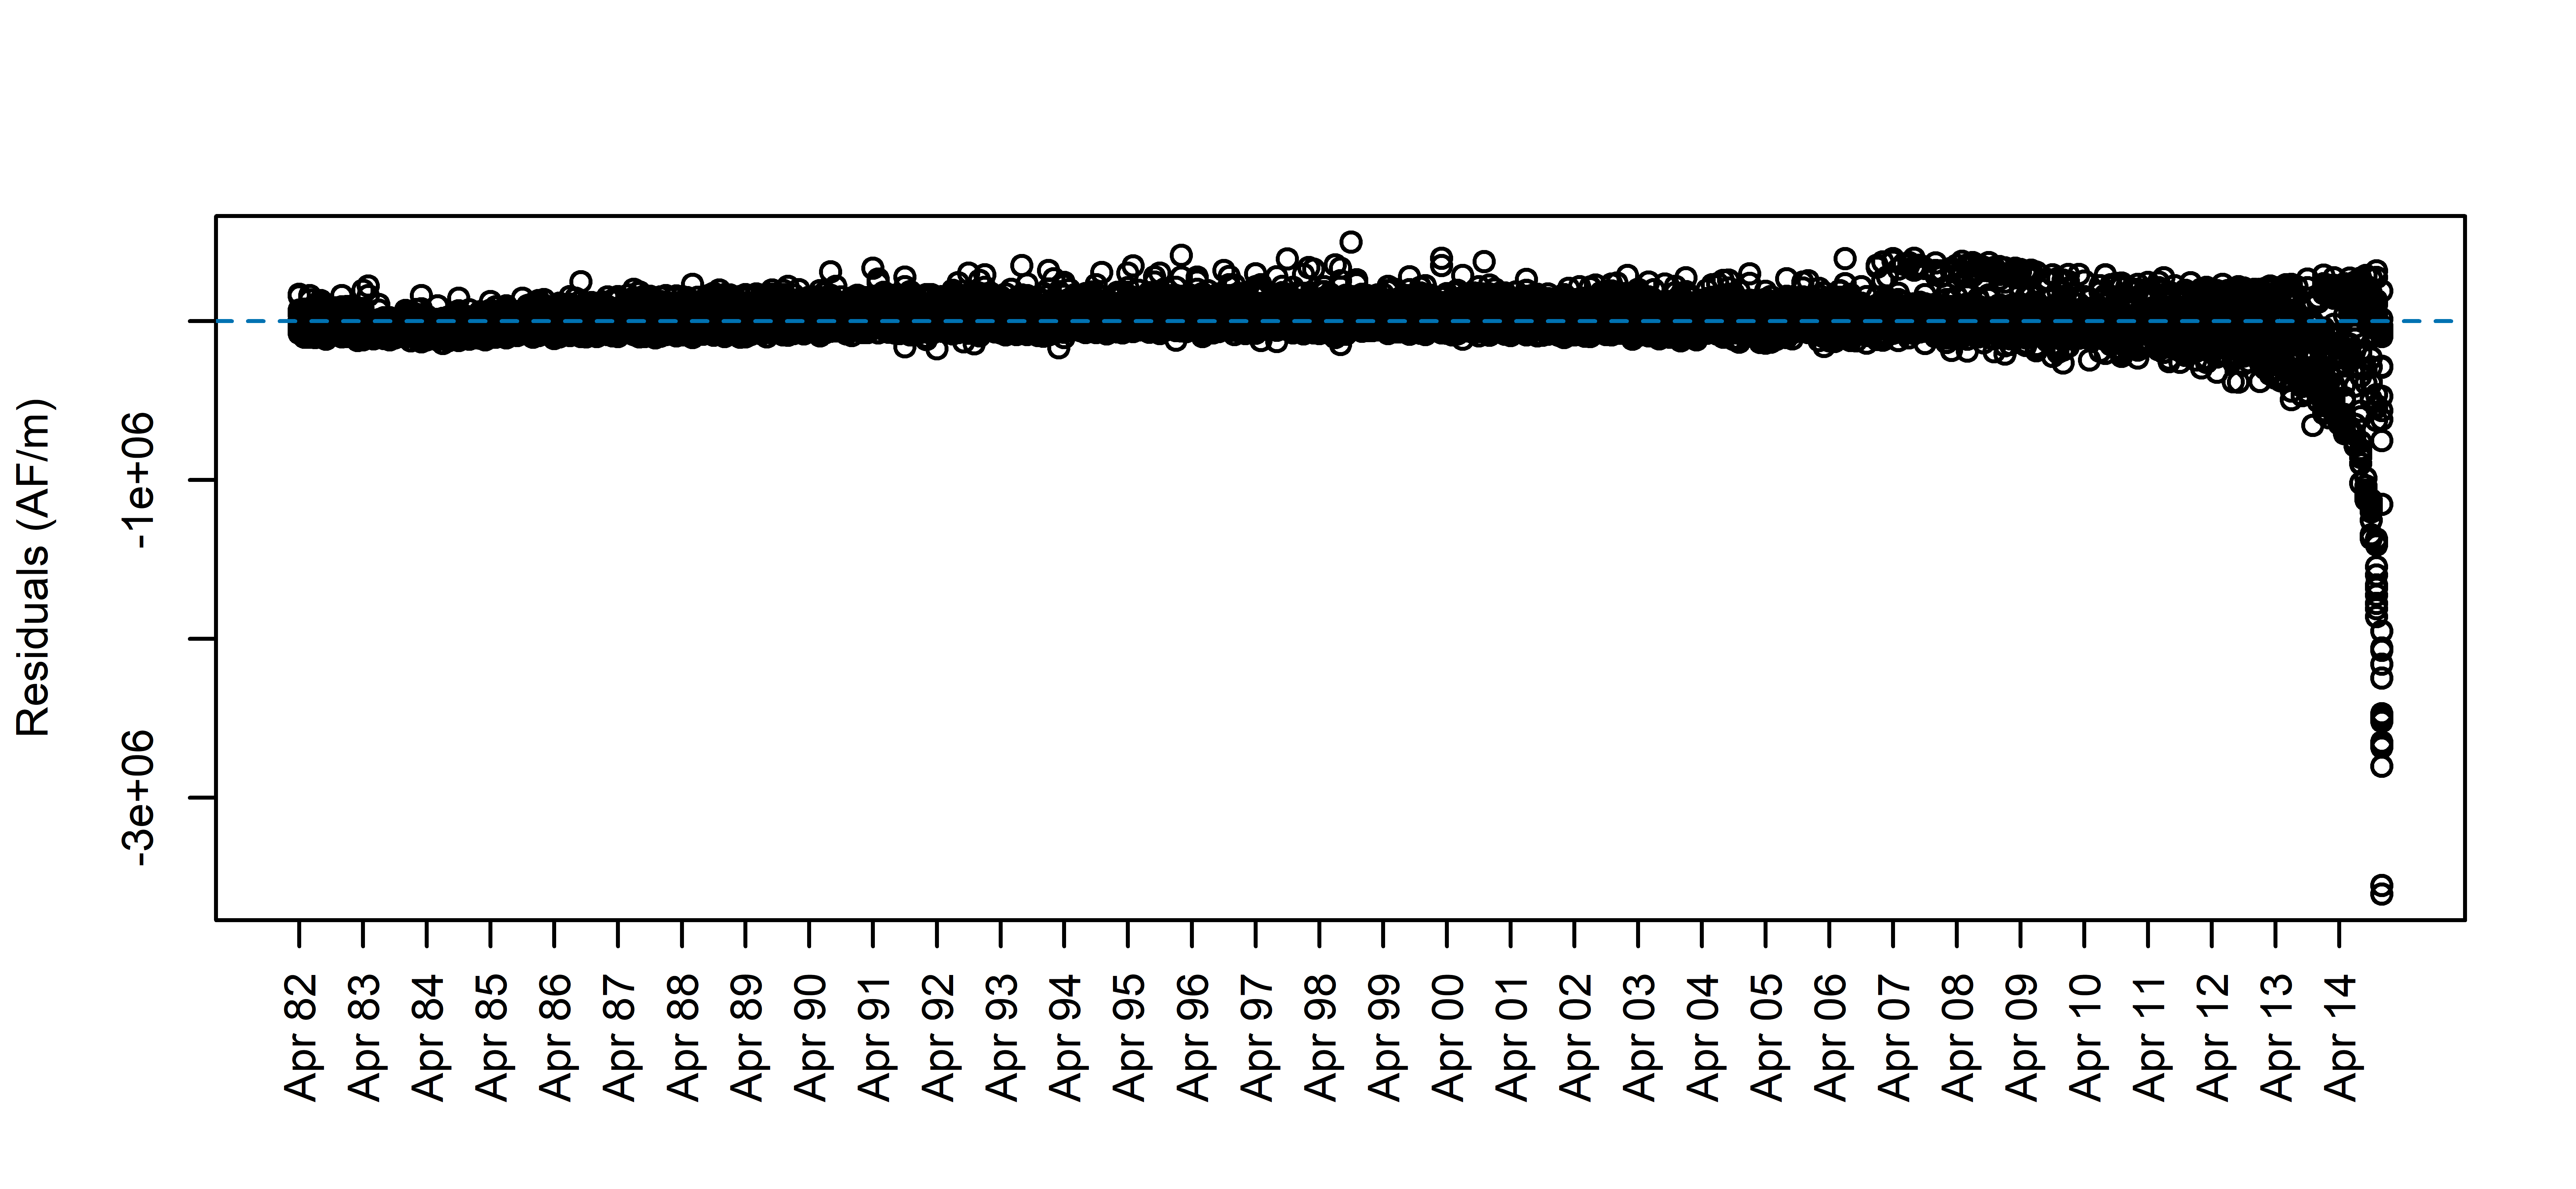
\includegraphics[width=\textwidth, trim={0 0 0 1cm}, clip=true]{plots/rplot22_lmlogo_residovertime_inc.png}
  		\caption{LM Incremental}
  		\label{fig:restimelm}
	\end{subfigure}% 
	\begin{subfigure}{.5\textwidth}
  		\centering
 		 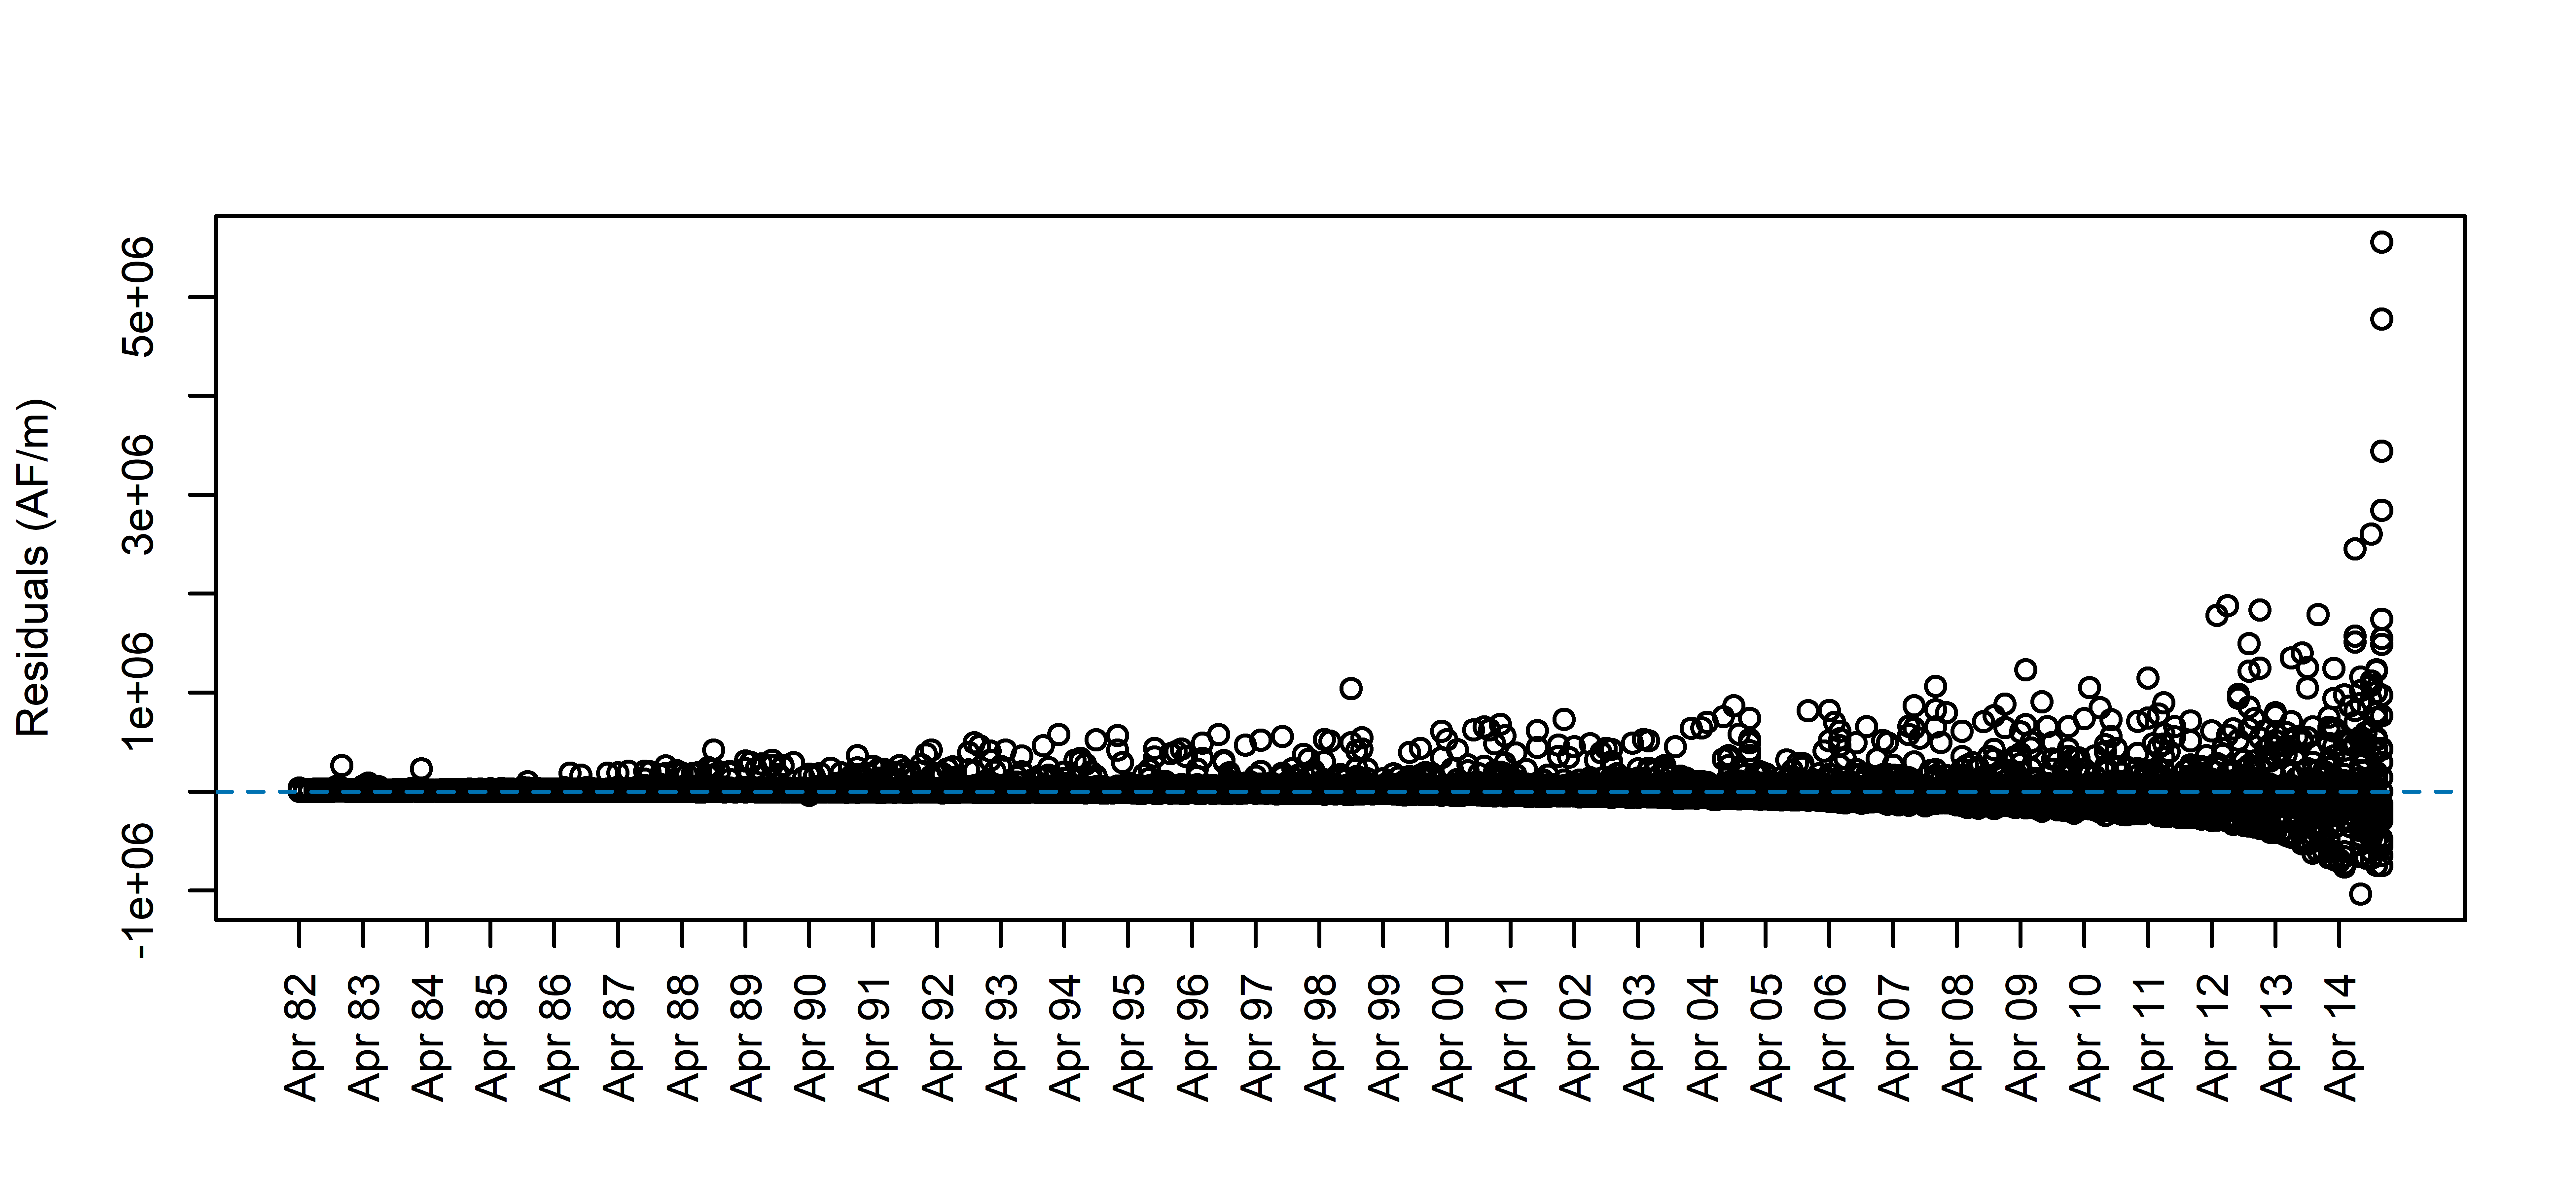
\includegraphics[width=\textwidth, trim={0 0 0 1cm}, clip=true]{plots/rplot22_glmlogo_residovertime_inc.png}
  		\caption{GLM Incremental}
  		\label{fig:restimeglm}
	\end{subfigure}% 
	\hfill
	\begin{subfigure}{.5\textwidth}
  		\centering
 		 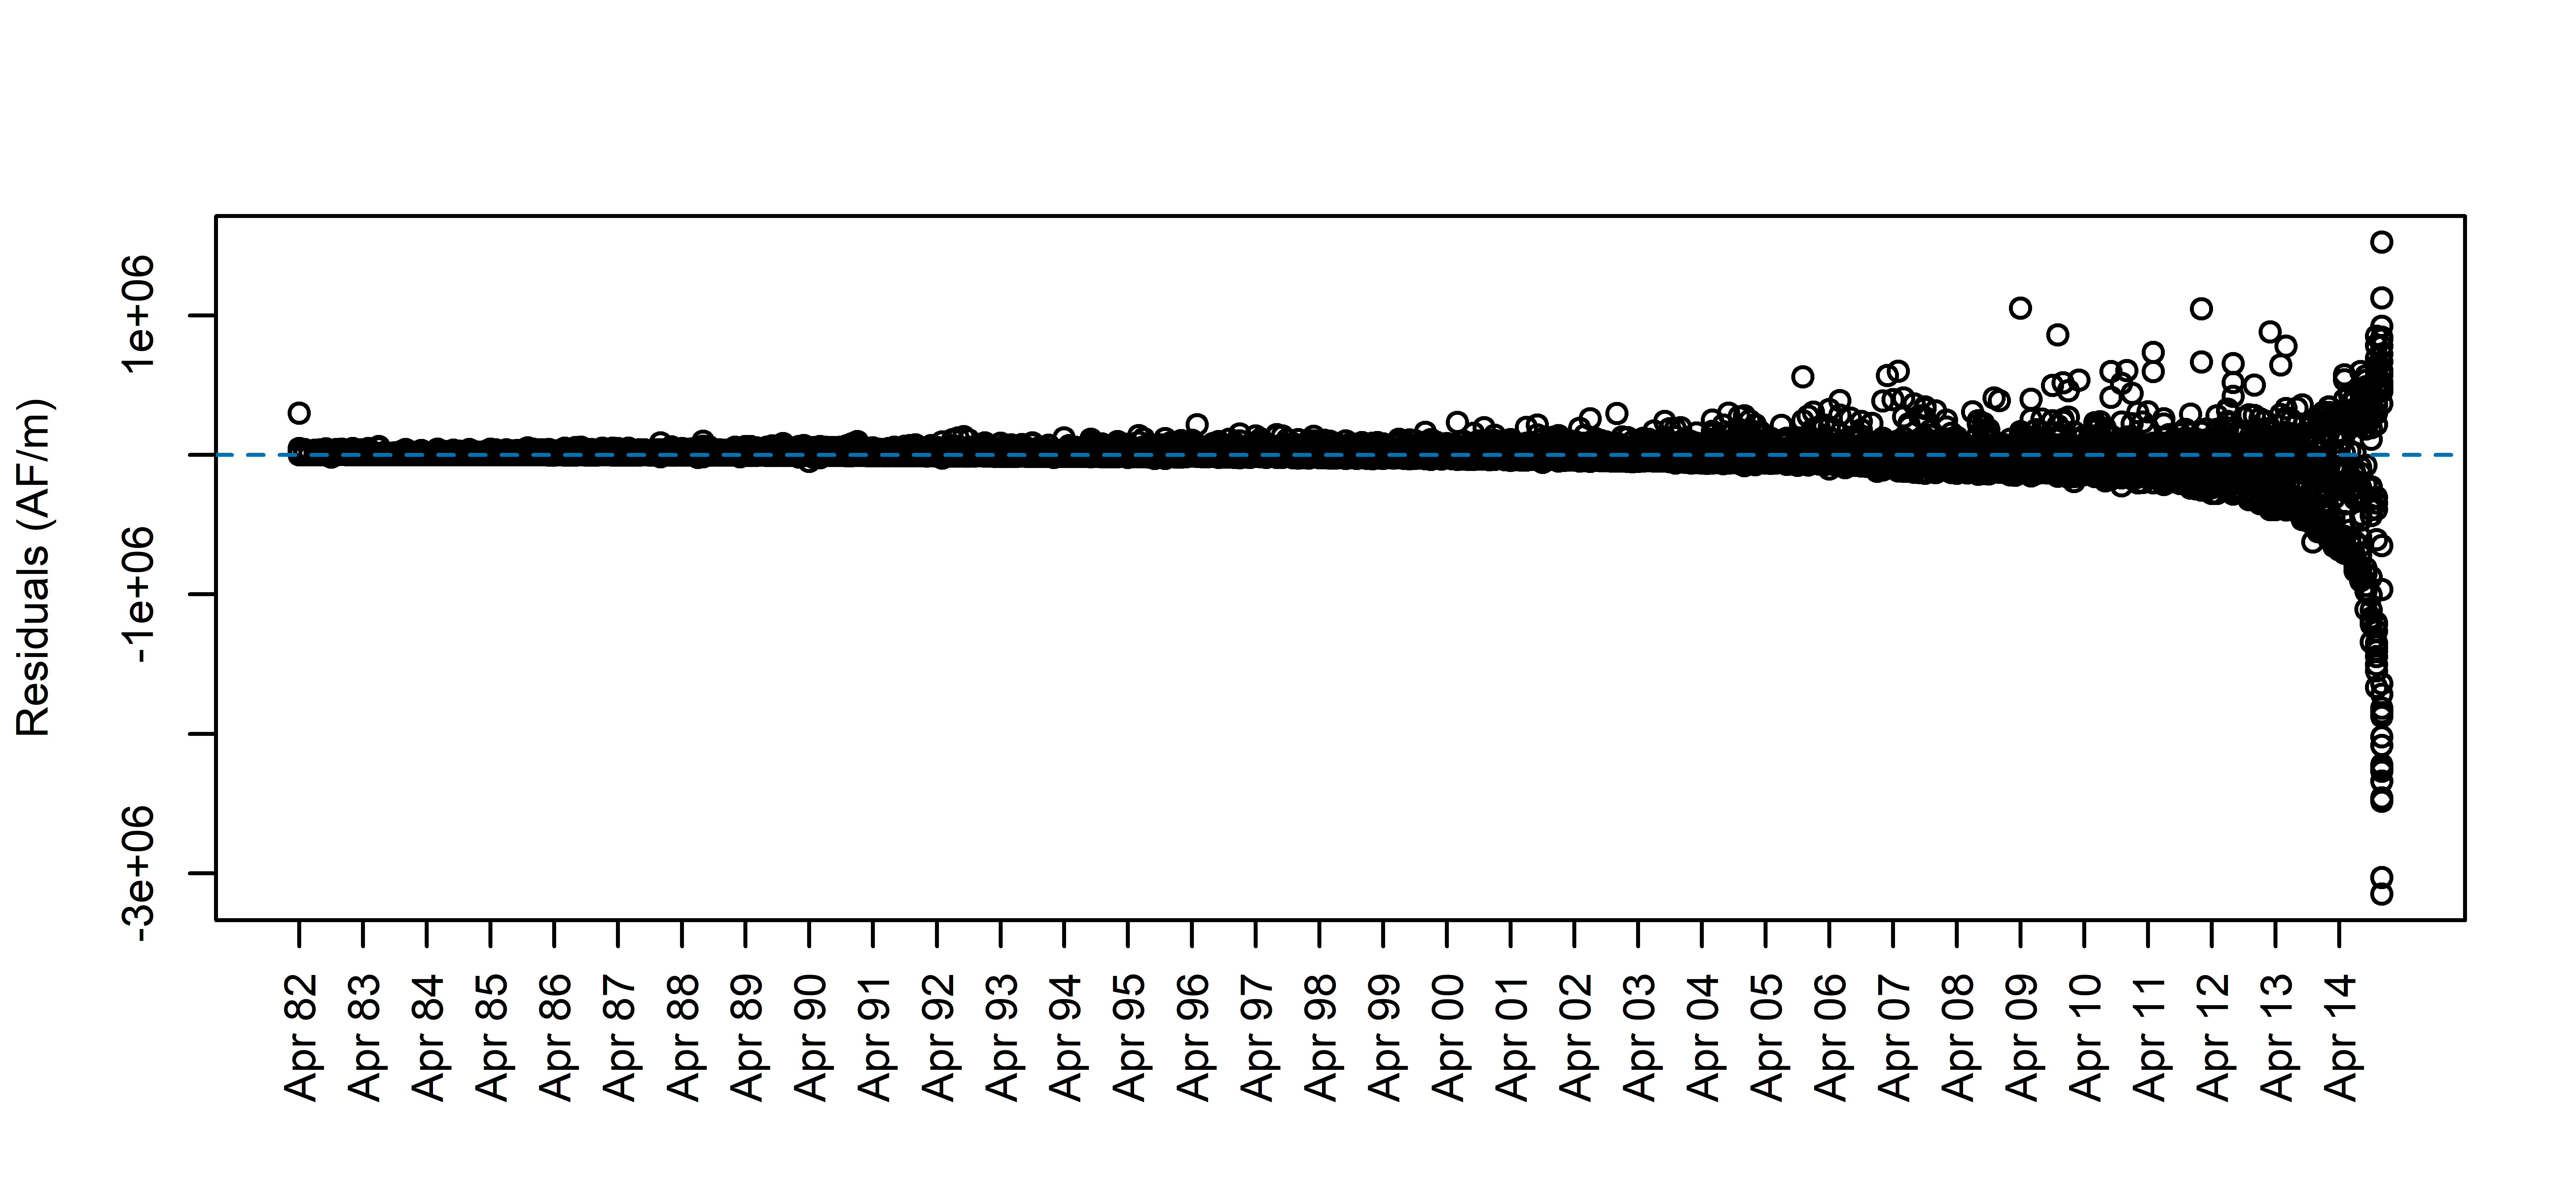
\includegraphics[width=\textwidth, trim={0 0 0 1cm}, clip=true]{plots/rplot22_rflogo_residovertime_inc.png}
  		\caption{RF Incremental}
  		\label{fig:restimerf}
	\end{subfigure}% 
	\begin{subfigure}{.5\textwidth}
  		\centering
  		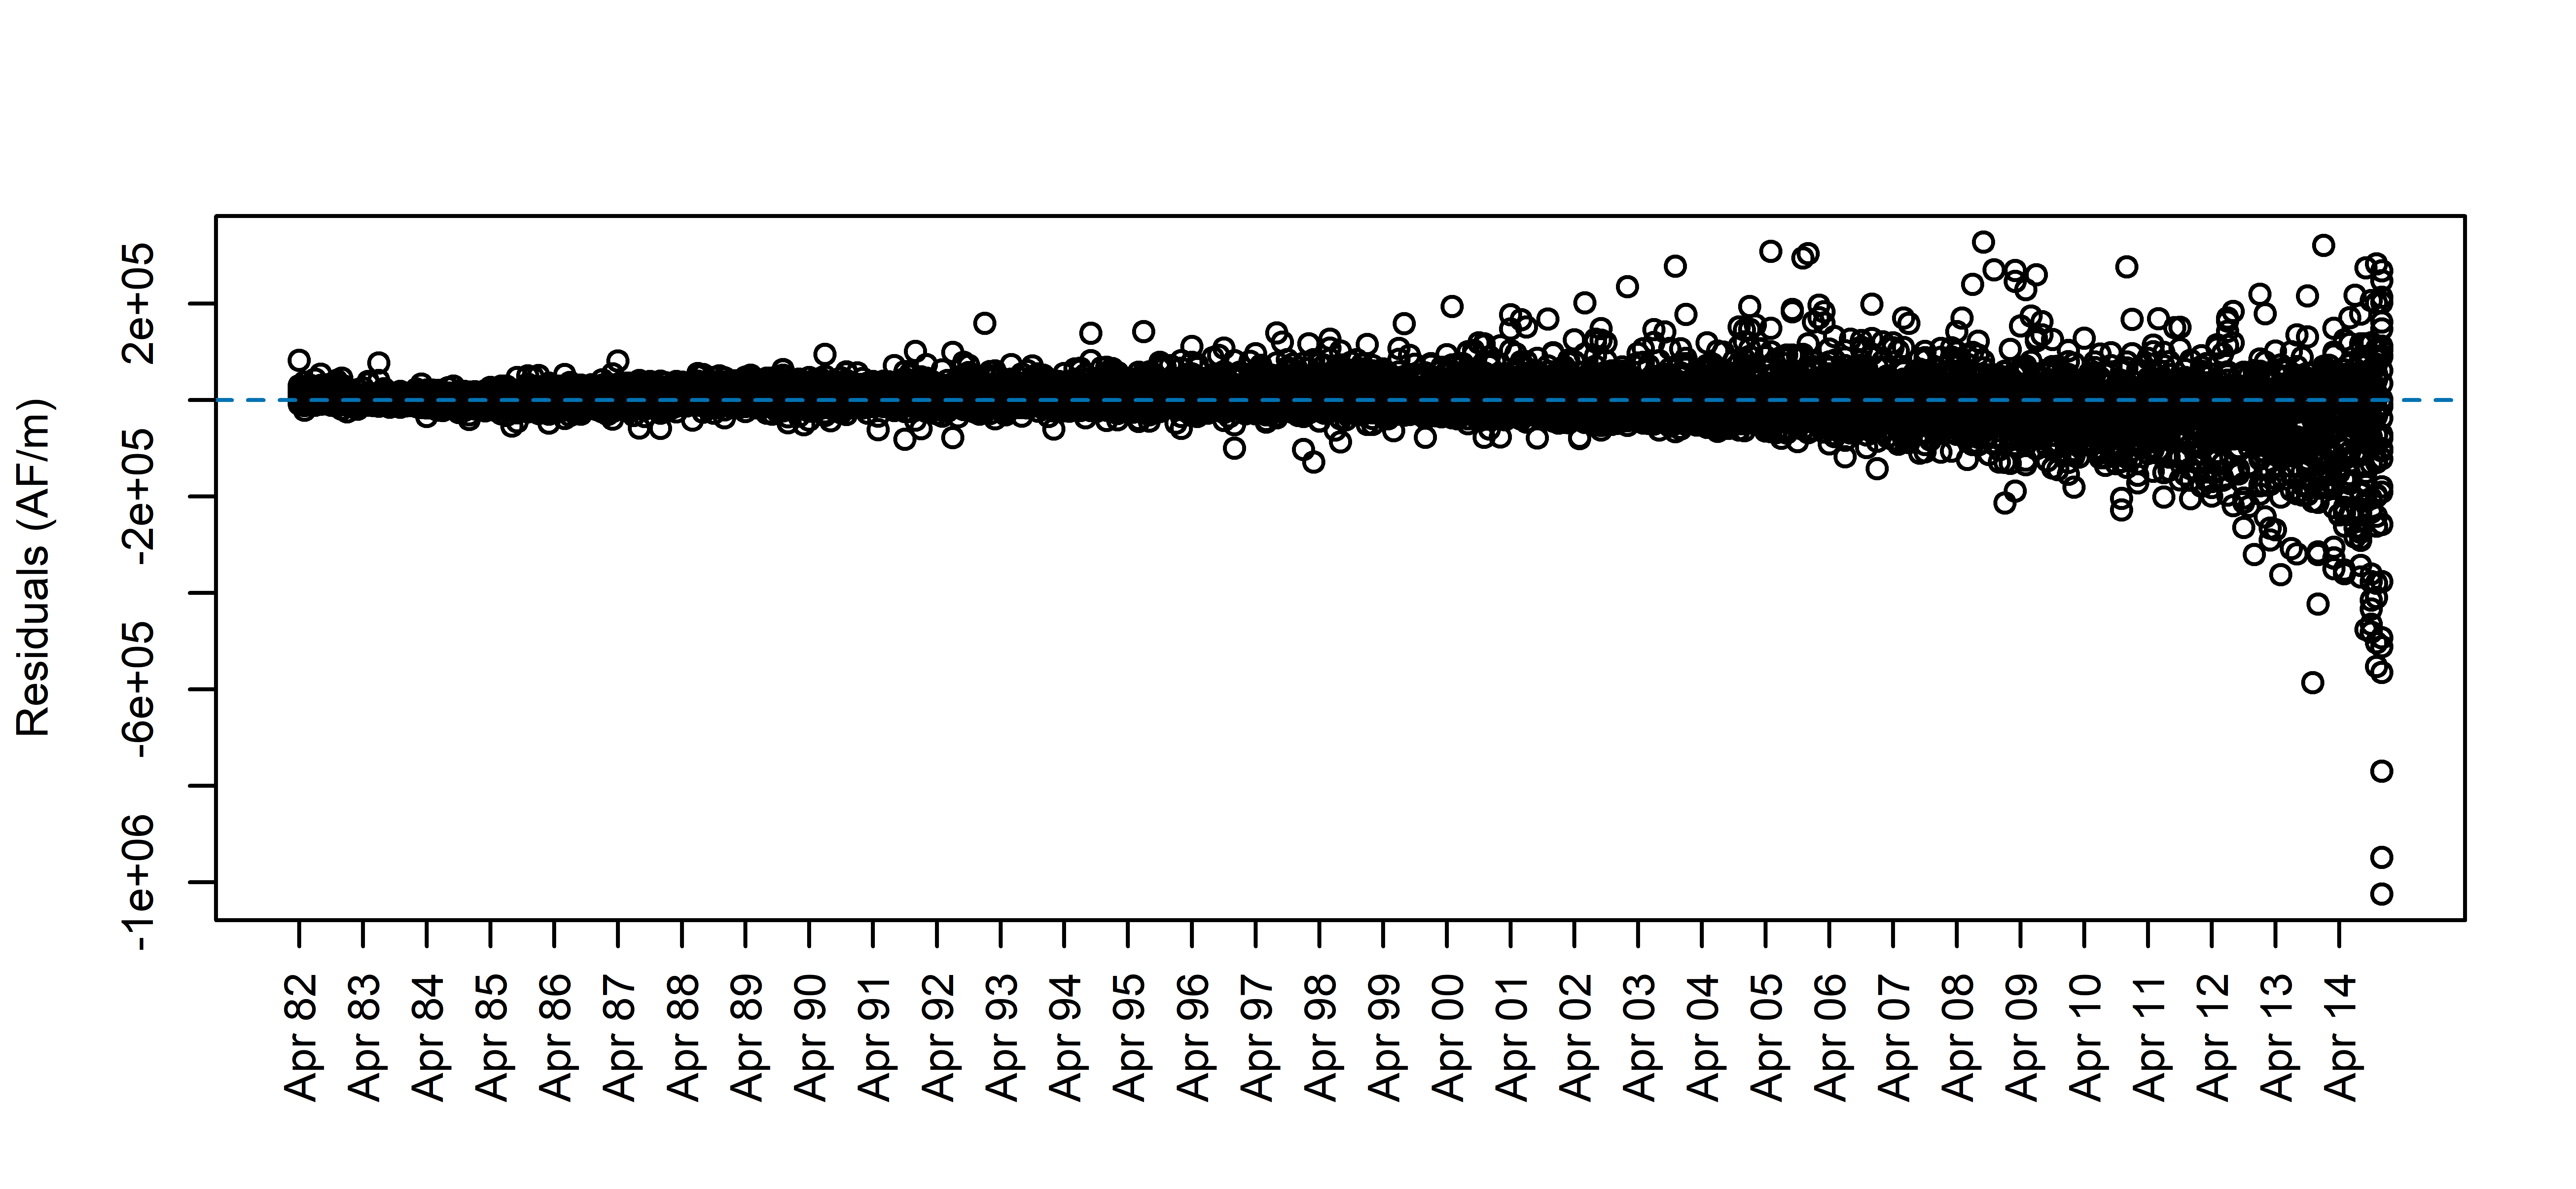
\includegraphics[width=\textwidth, trim={0 0 0 1cm}, clip=true]{plots/rplot22_nnlogo_residovertime_inc.png}
  		\caption{NN Incremental}
  		\label{fig:restimenn}
	\end{subfigure}
	\caption{}
	\label{fig:resovertime}
\end{figure}

In the NSE, the NN incremental model provides the best model performance, therefore, we will now abandon the comparative analysis and examine the spatial distribution of this model.
%-----------------------------------------------
\subsection{Spatial Distribution of Errors}
Figures \ref{fig:incbr2plus} and \ref{fig:aggincbr2comp} show the bR\textsuperscript{2} values for the 67 basins in this study. As expected, the model's ability to predict unimpaired flow varies across California. The model performs better at basins  lower in the network (i.e., have a higher hierarchy). This could be due to: (1) the basins with higher hierarchies generally have larger flows and the model is trained with a squared error loss that penalizes large errors more harshly; or (2) there was substantial value in having flow information upstream (i.e, the decline is error is due to having incremental basins). 

\begin{figure}
	\centering
	\begin{subfigure}{.5\textwidth}
  		\centering
 		 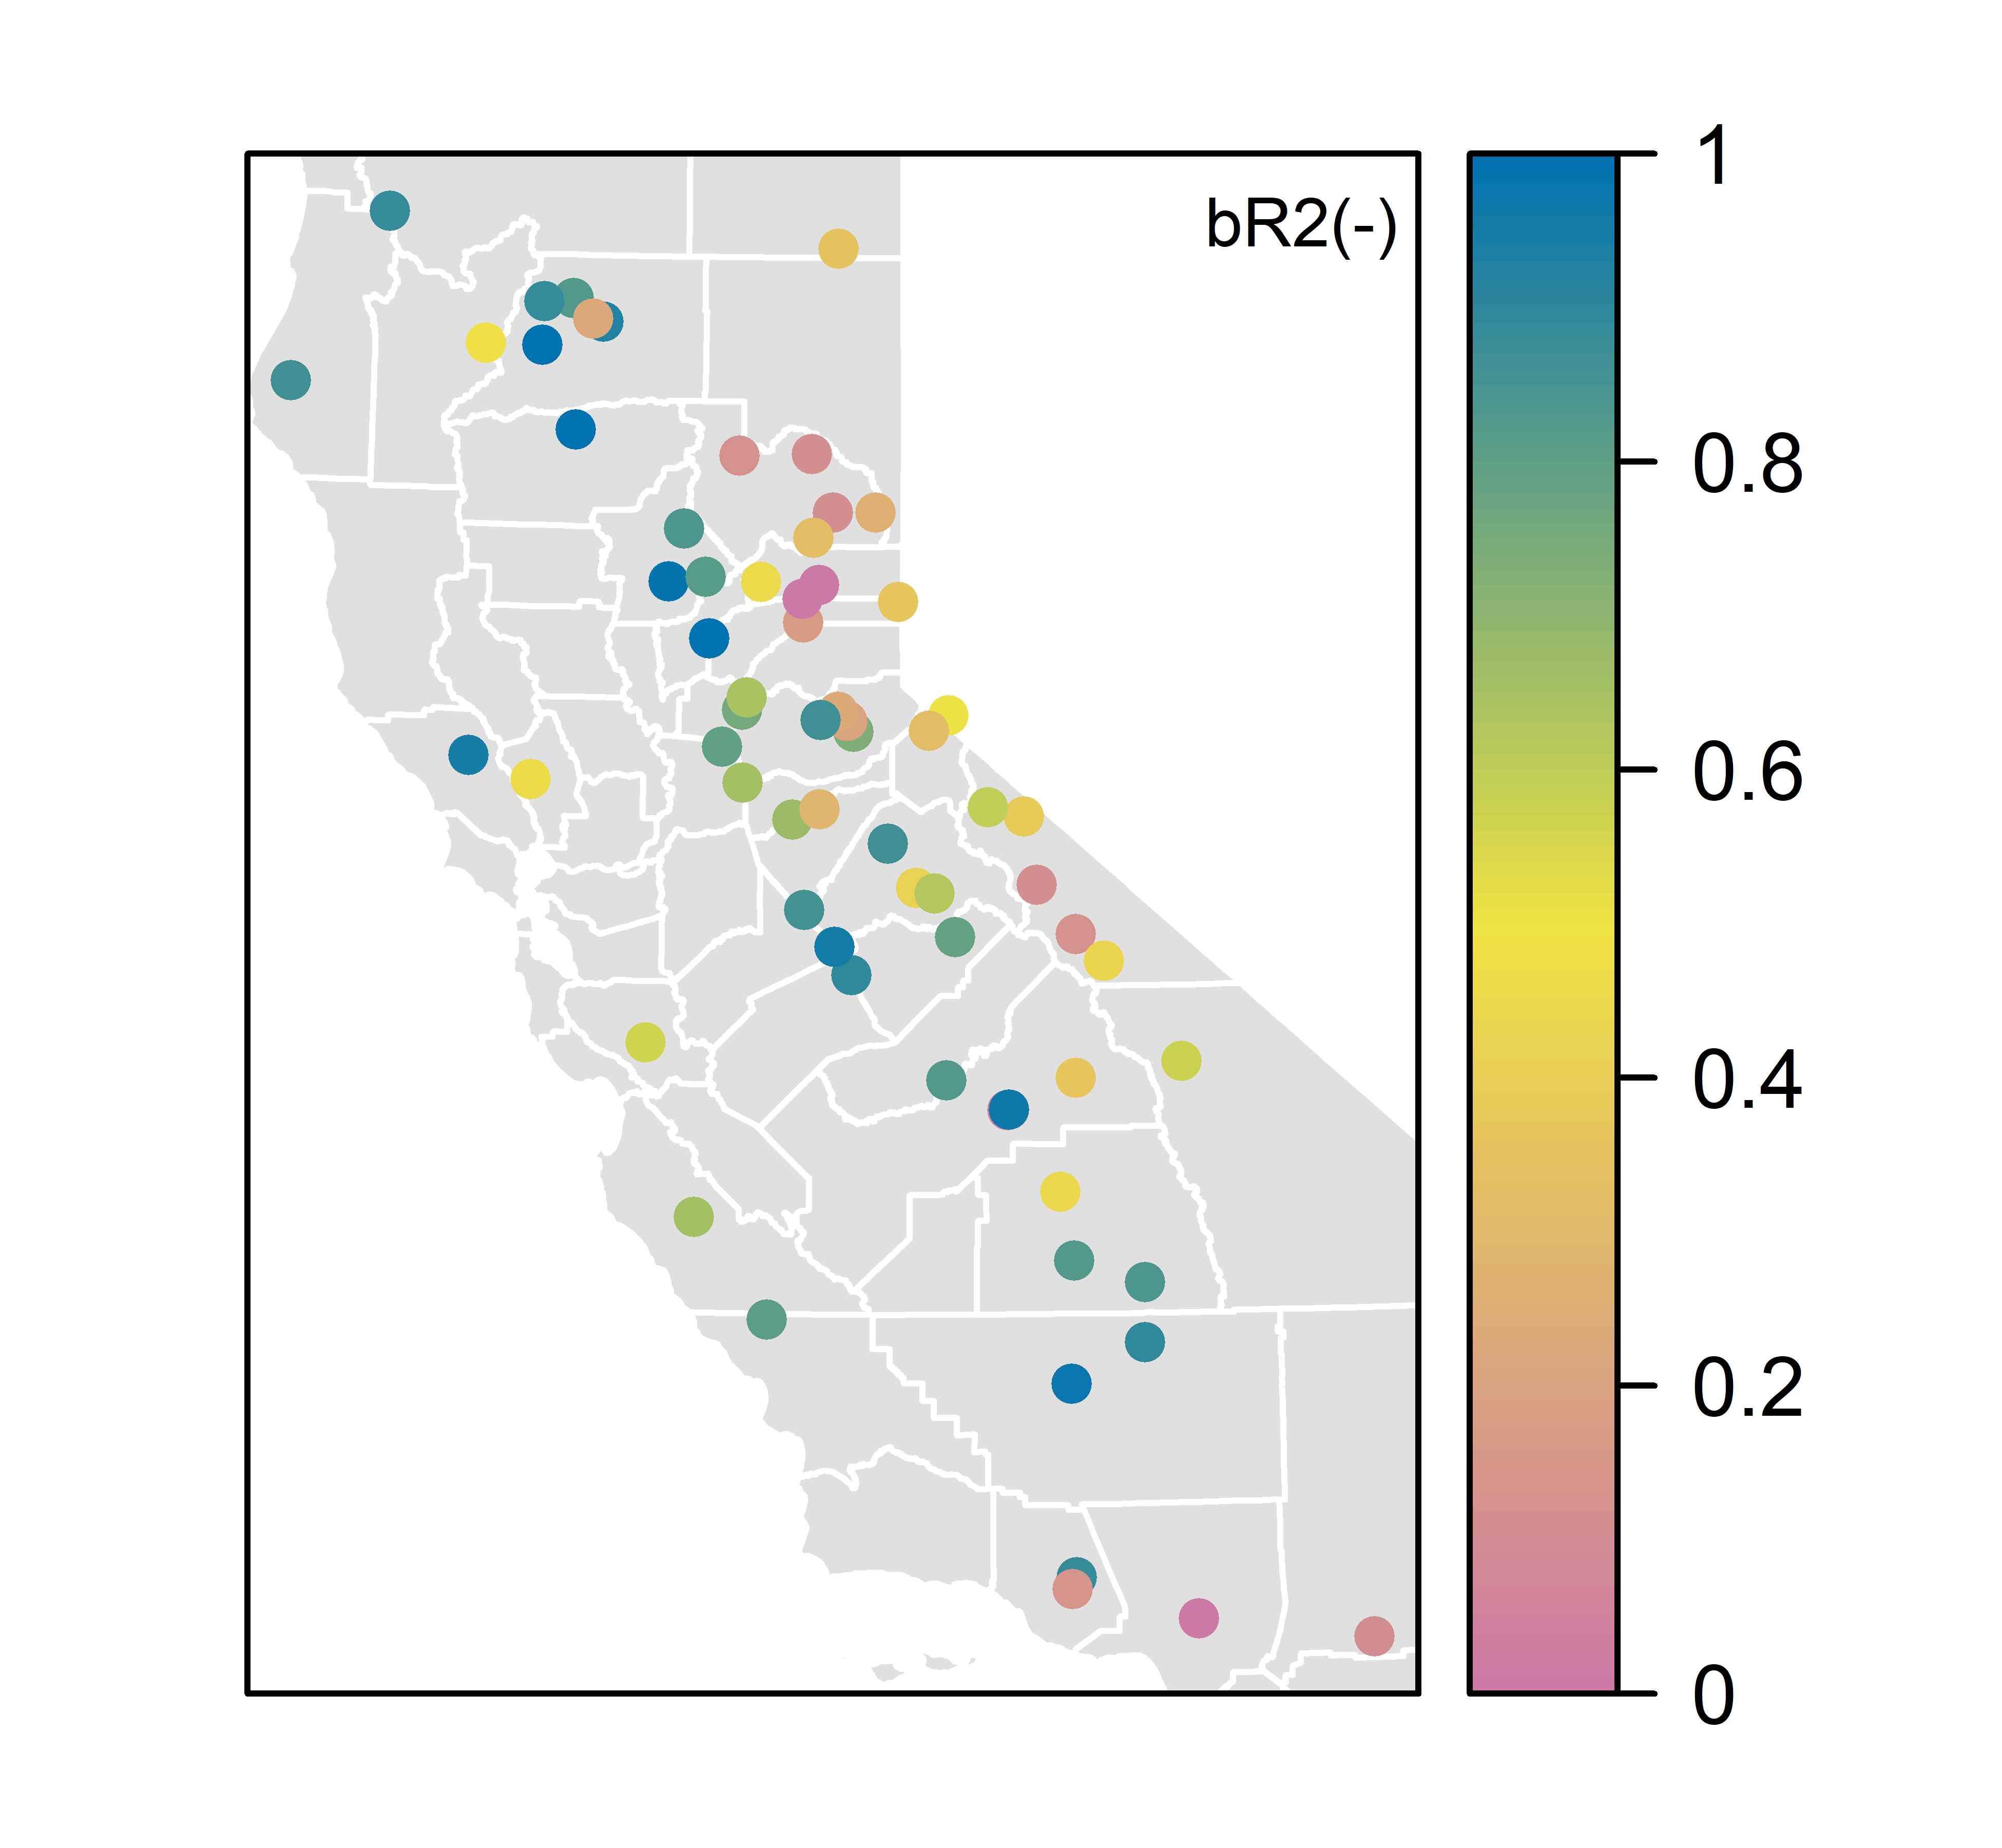
\includegraphics[width=\textwidth, trim={0 0 0 0}, clip=true]{plots/rplot28_br2map_nn_inc.png}
  		\caption{Test Set Error}
	\end{subfigure}% 
	\begin{subfigure}{.5\textwidth}
  		\centering
 		 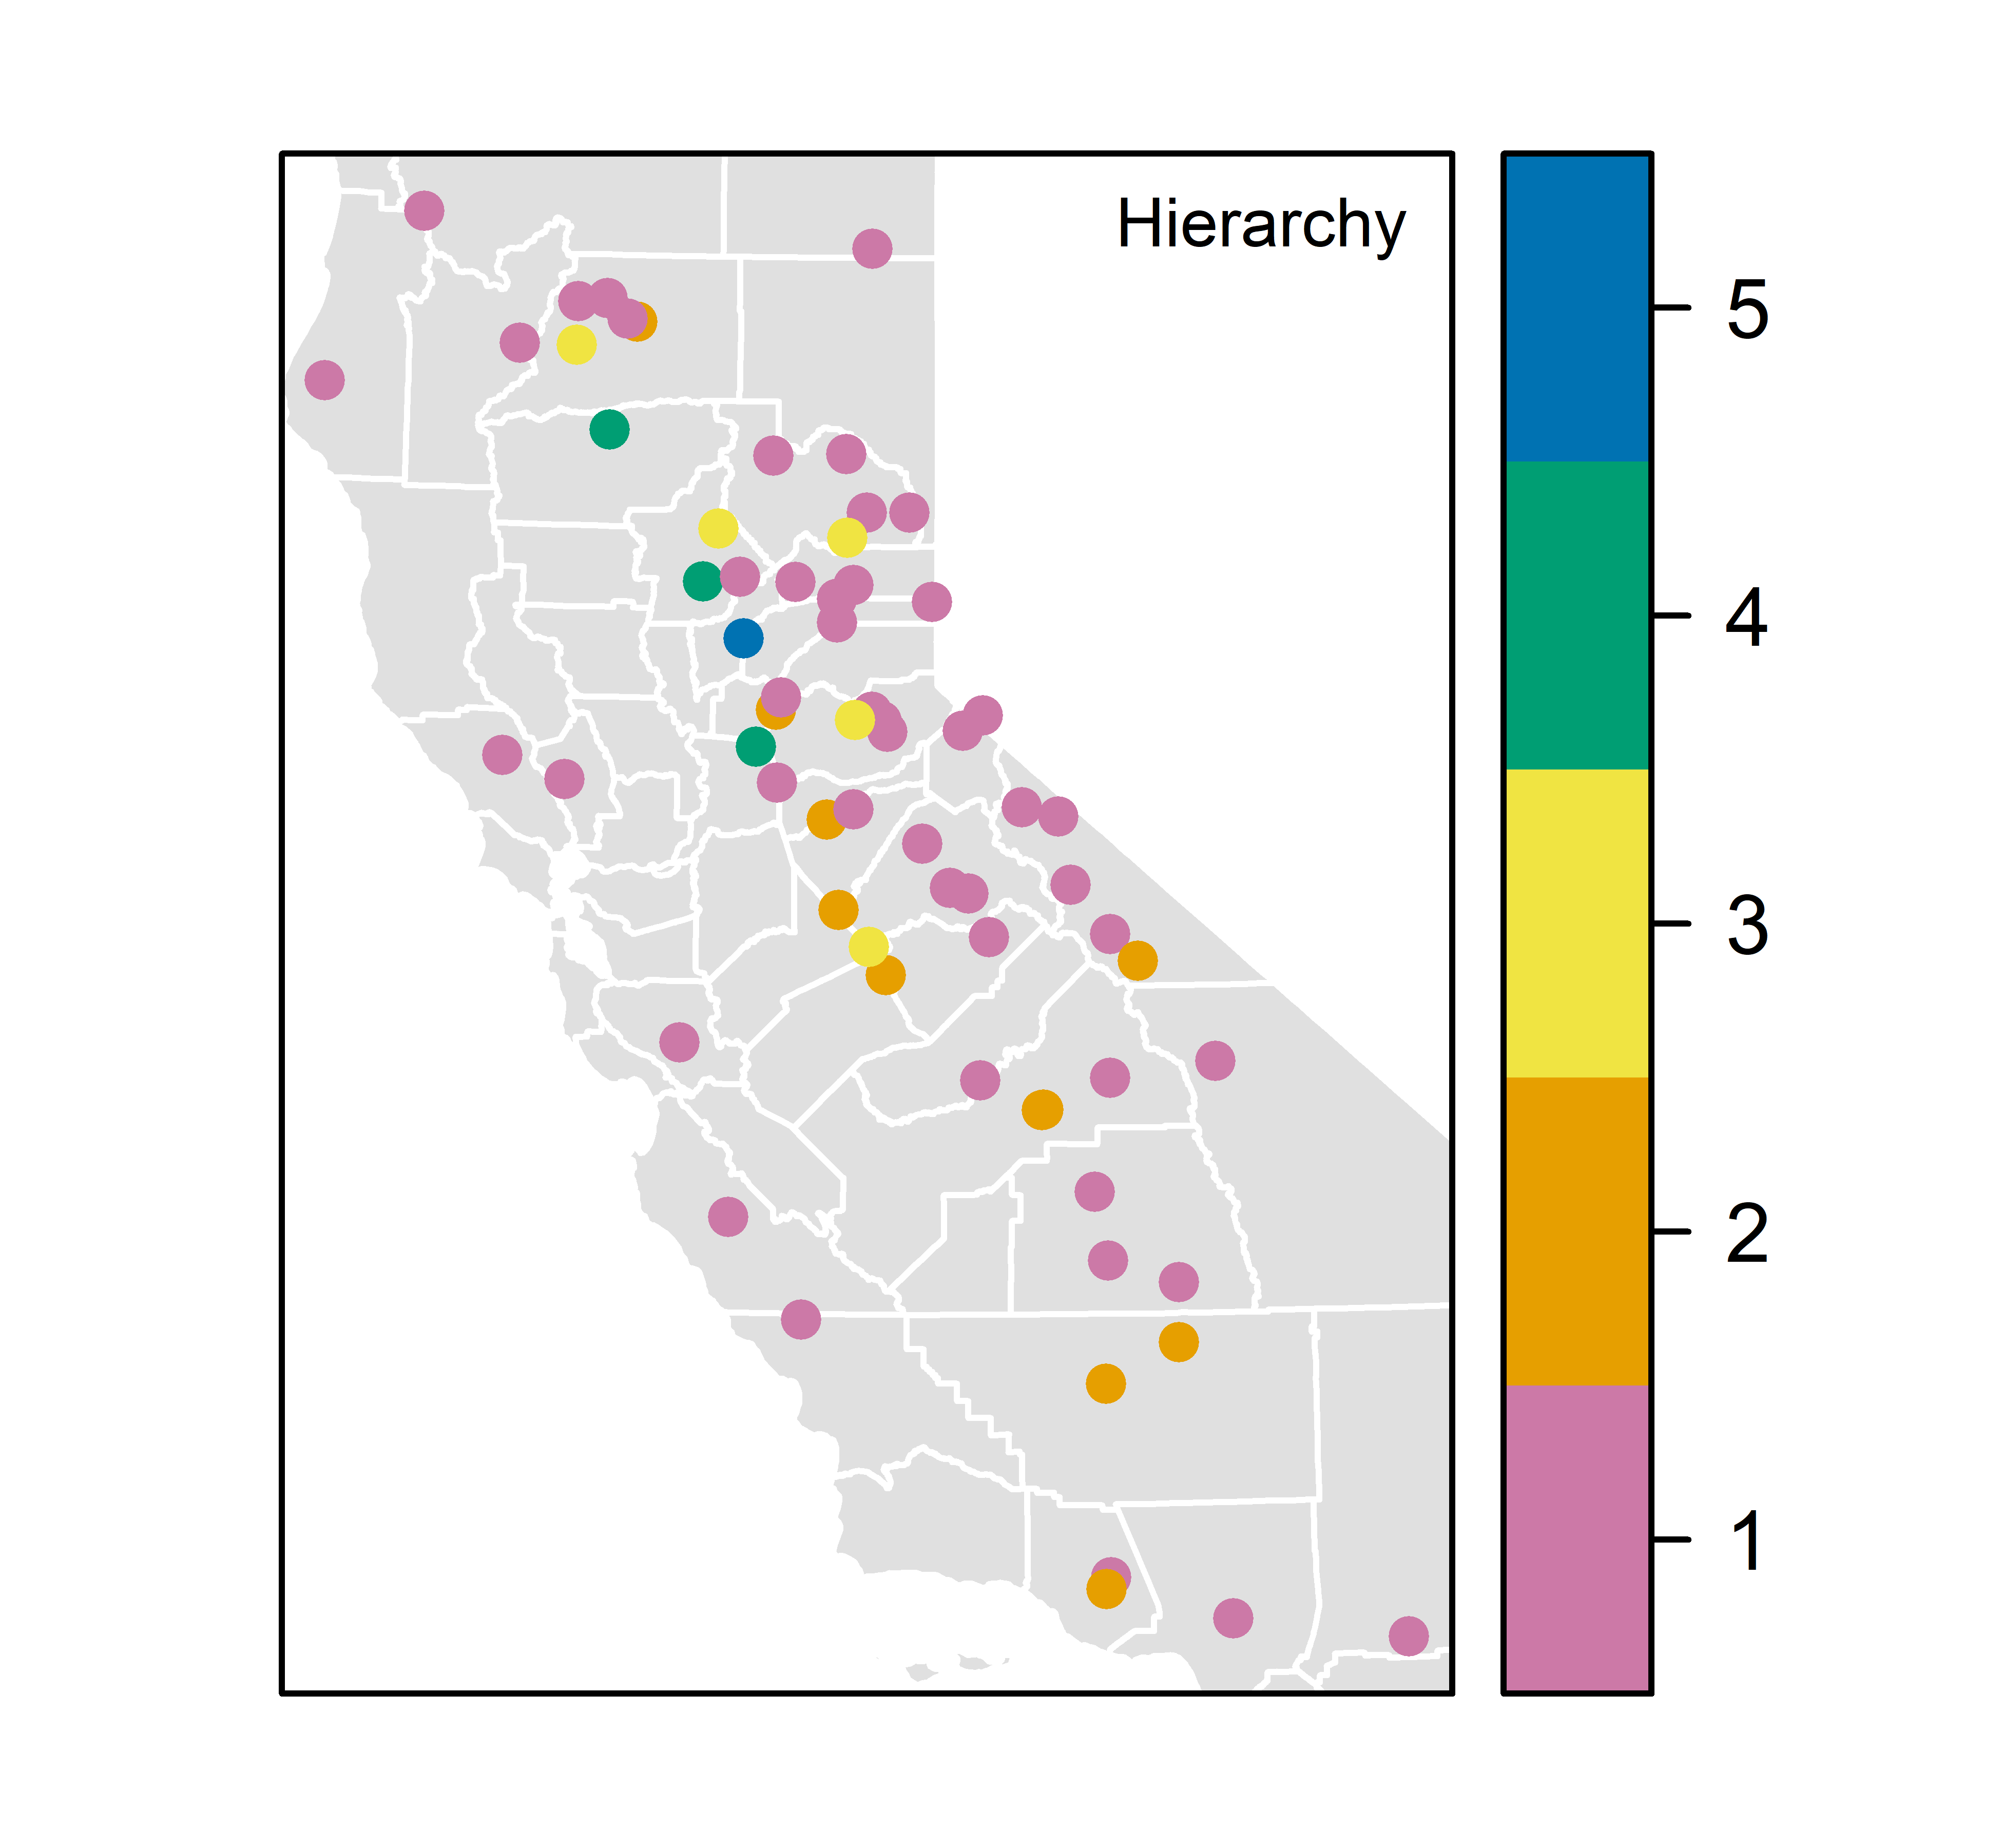
\includegraphics[width=\textwidth, trim={0 0 0 0}, clip=true]{plots/rplot210_hierarchies.png}
  		\caption{Basin Hierarchies}
	\end{subfigure}% 
	\hfill
	\caption{The spatial distribution of errors. (a) The bR\textsuperscript{2} error is not random and follows a line down the middle of California, and it somewhat follows the basin hierarchies. (b) The basins are not evenly distributed between the hierarchies; the lower the hierarchy the more basins in this study. Altogether, the lower the basin is in the network (i.e., the higher its hierarchy), the better the model performs.}
	\label{fig:incbr2plus}
\end{figure}

\begin{figure}
	\centering
	\begin{subfigure}{.5\textwidth}
  		\centering
 		 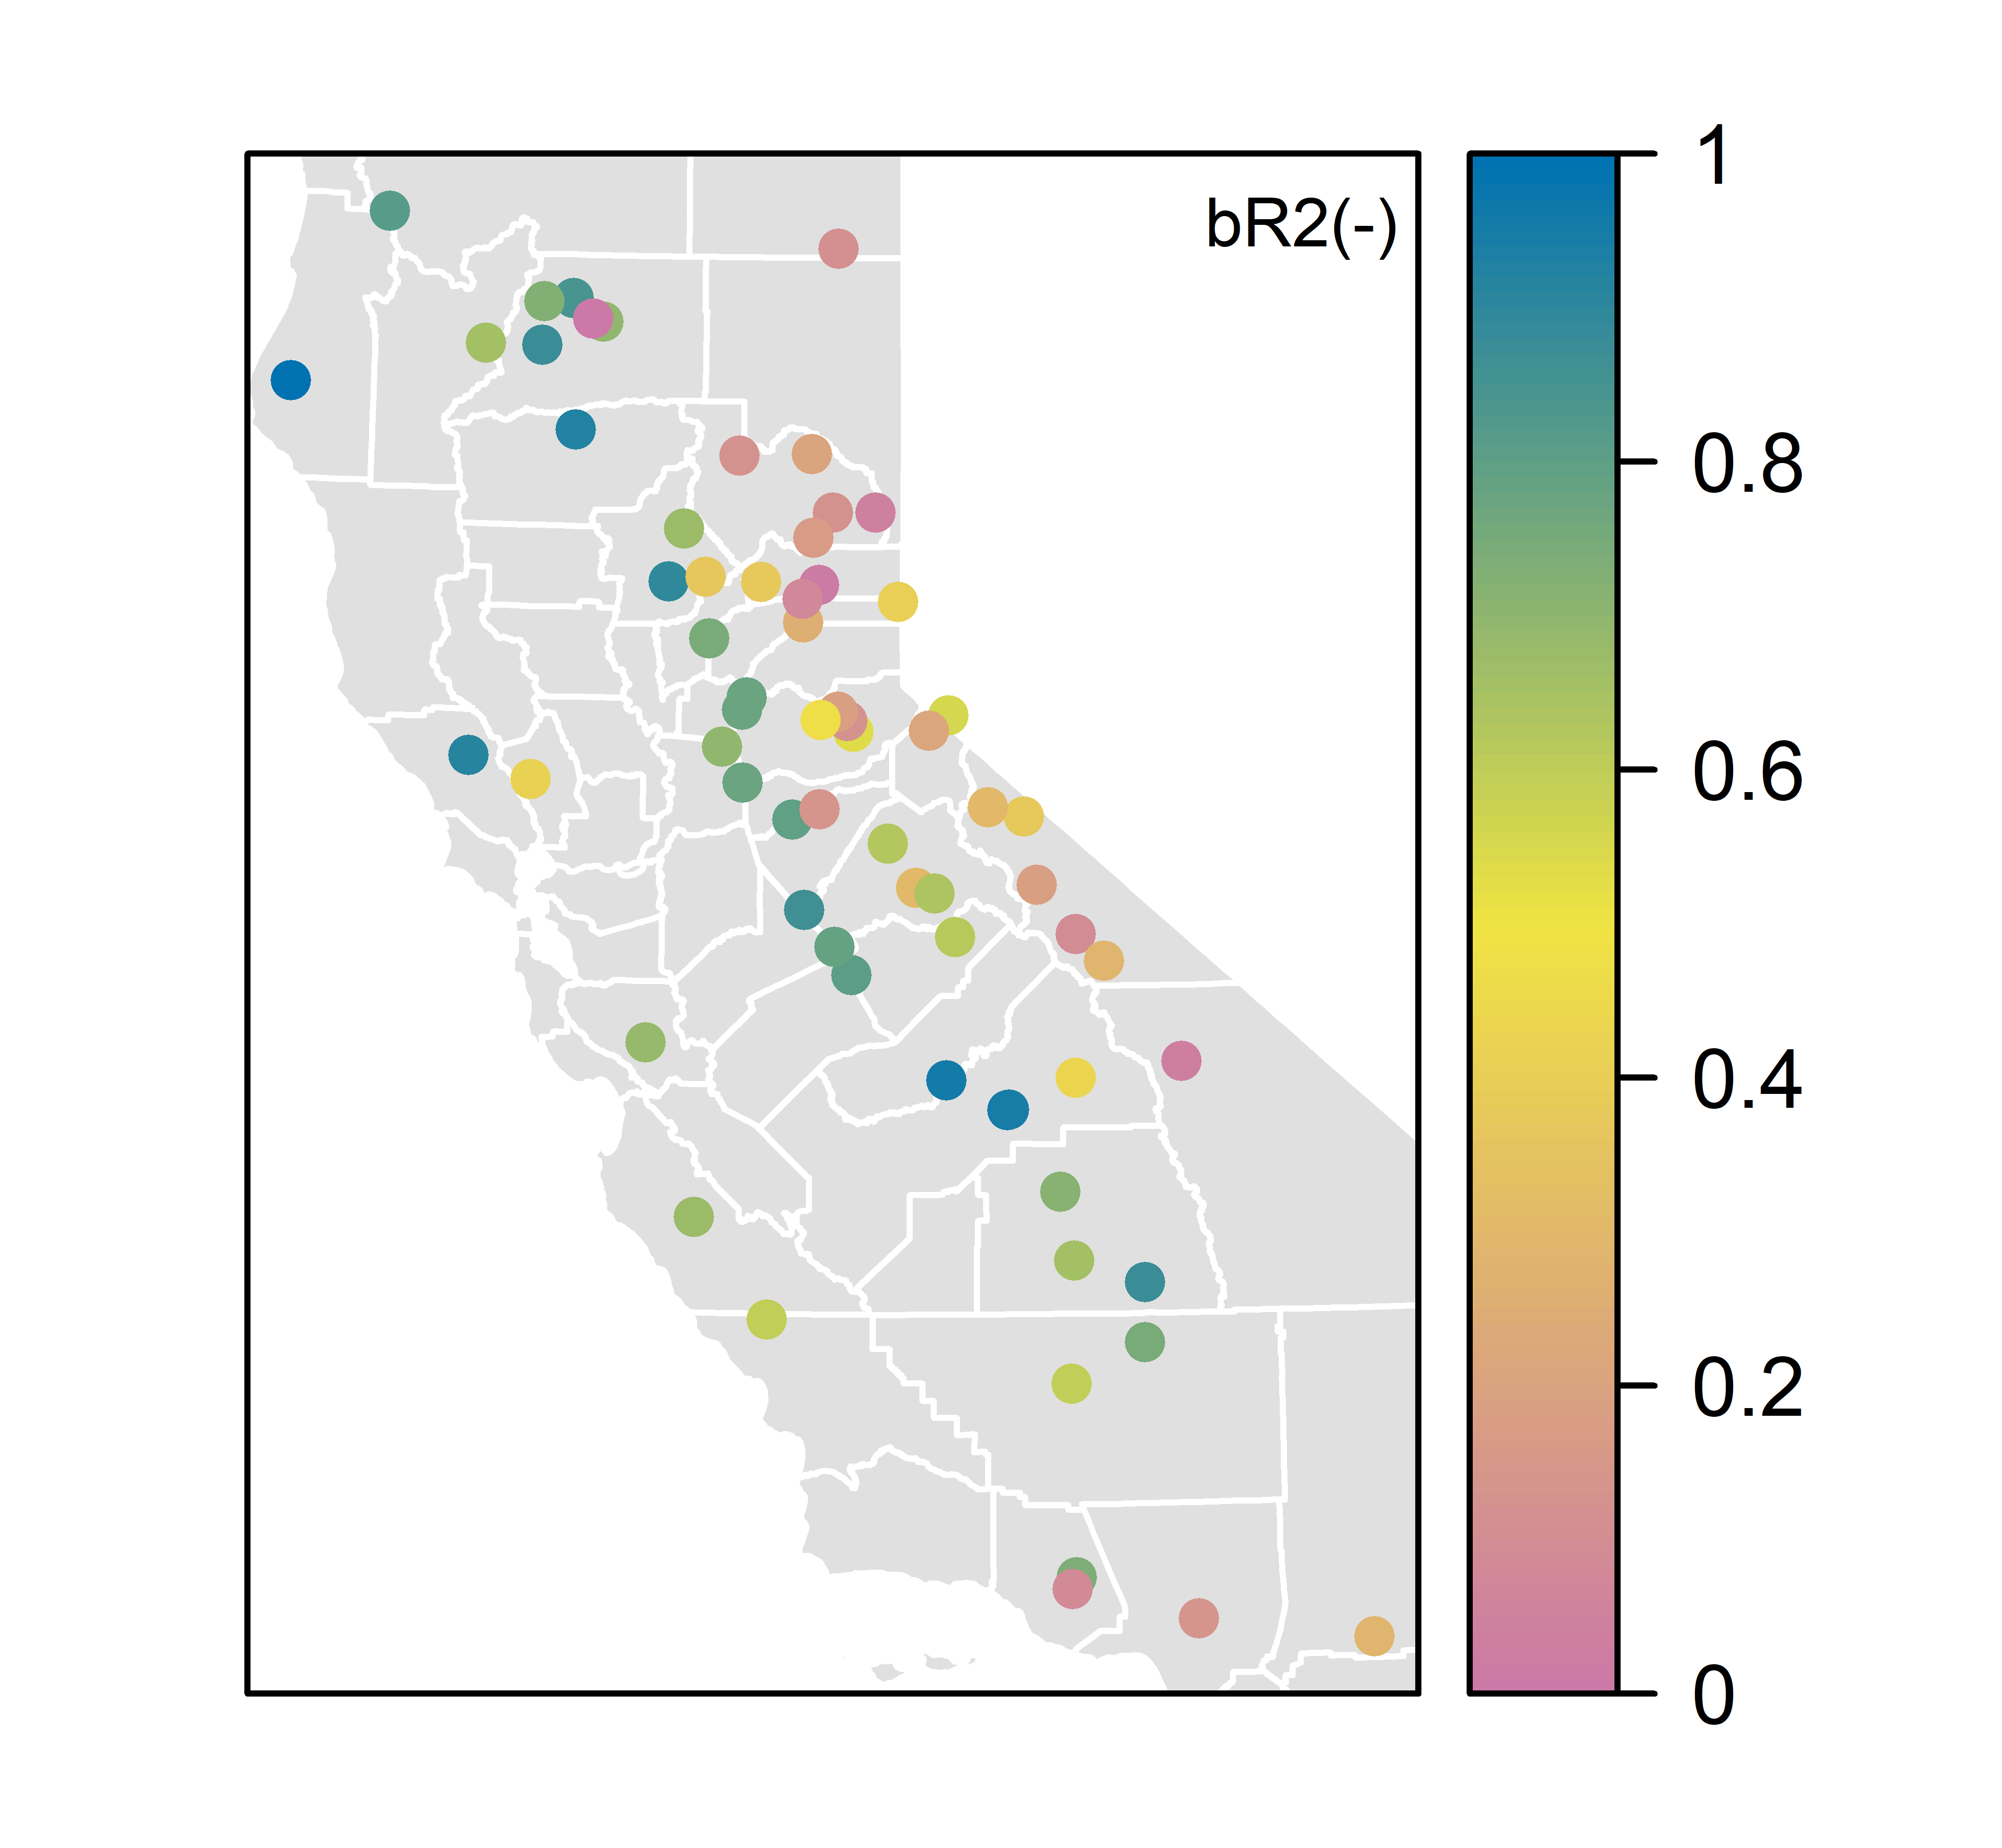
\includegraphics[width=\textwidth, trim={0 0 0 0}, clip=true]{plots/rplot28_br2map_nn_agg.png}
  		\caption{NN Aggregate}
	\end{subfigure}% 
	\begin{subfigure}{.5\textwidth}
  		\centering
 		 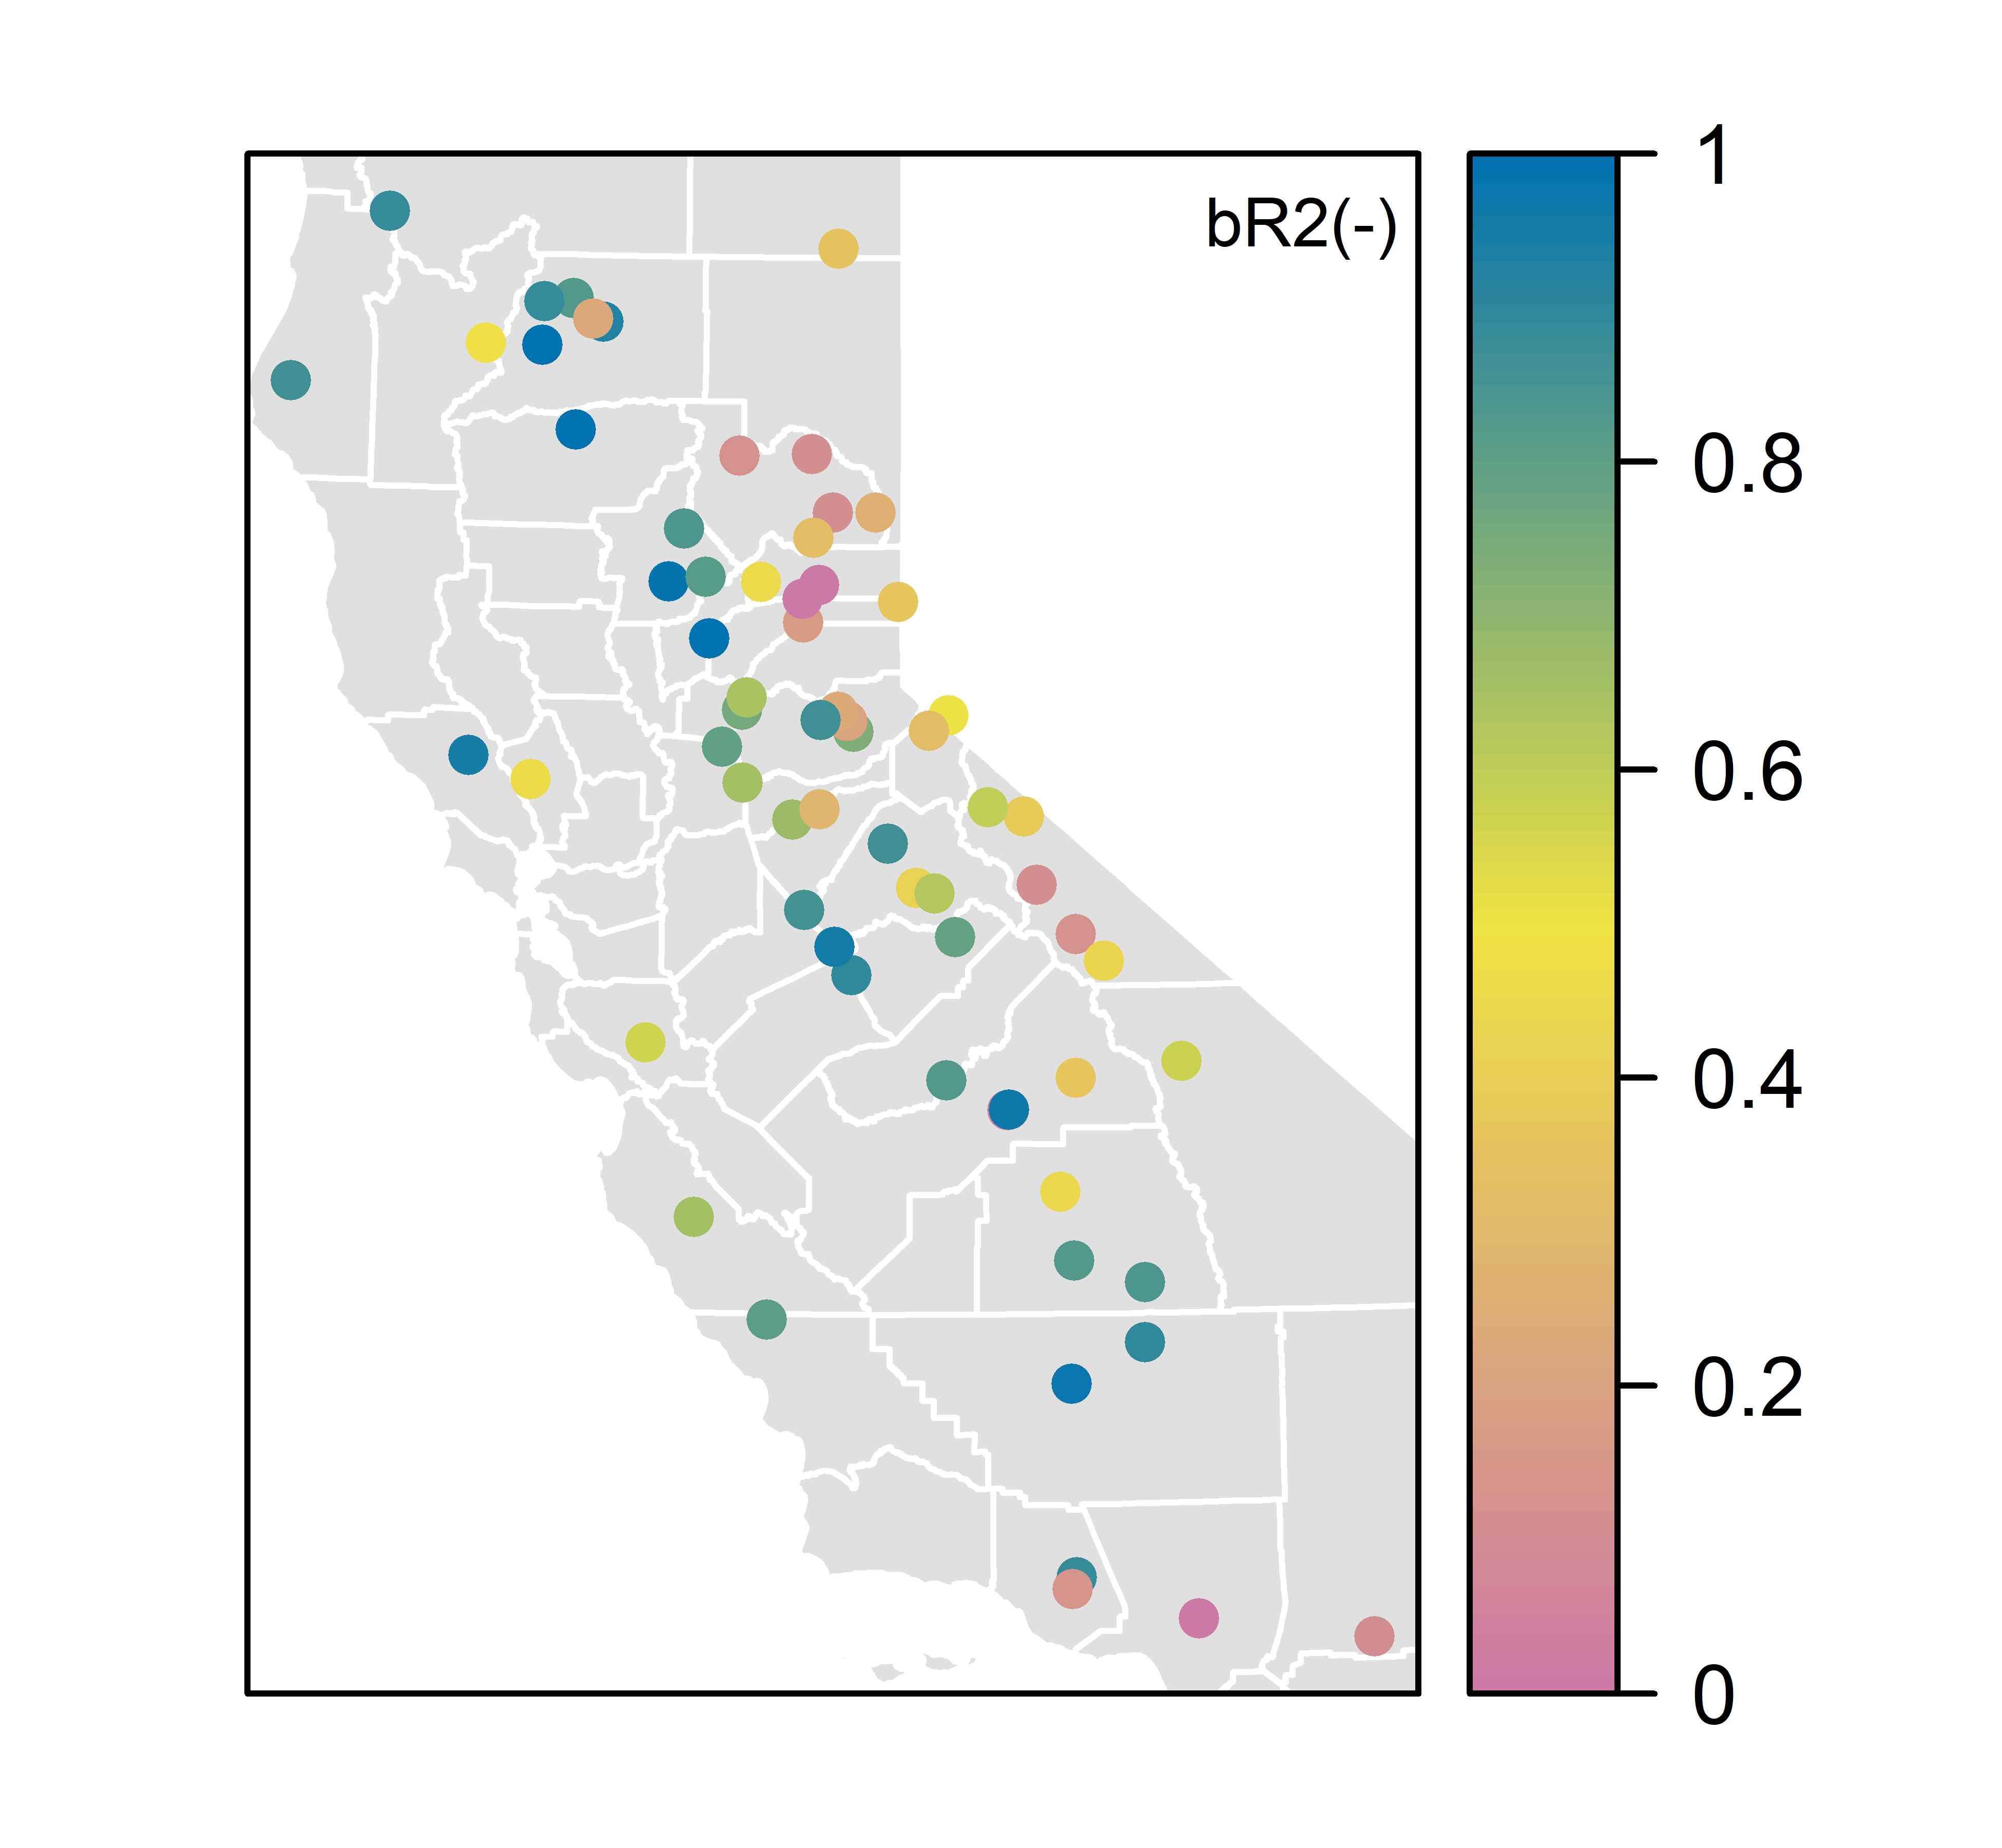
\includegraphics[width=\textwidth, trim={0 0 0 0}, clip=true]{plots/rplot28_br2map_nn_inc.png}
  		\caption{NN Incremental}
	\end{subfigure}% 
	\hfill
	\caption{The aggregate and incremental basins perform very similarly when there isn't any information upstream (i.e., hierarchy=1). However, when we introduce information upstream (i.e., hierarchy=2,3,4, and 5) the incremental basins can perform much better than the aggregate.}
	\label{fig:aggincbr2comp}
\end{figure}

Figures \ref{fig:br2dotchartcomp} and \ref{fig:br2boxplotcomp} show that when there is no flow information upstream (i.e., hierarchy=1) there is not much difference in the performance of incremental and aggregate models. However, when we introduce increasingly more information upstream (i.e., hierarchy=2,3,4, and 5) the NN incremental model can perform much better than the NN aggregate model. Even though the data set is smaller in the basins lower in the network, we can conclude that, the model is performing better at these basins due to information upstream and not just due to its higher flows and the loss function. 

\begin{figure}
  	\centering
 	 \includegraphics[width=0.9\textwidth, trim={0 0 0 0}, clip=true]{plots/rplot211_bR2dotchart_comp.png}
  	\caption{Basin bR\textsuperscript{2} performance in order.}
  	\label{fig:br2dotchartcomp}
\end{figure}

\begin{figure}
  	\centering
 	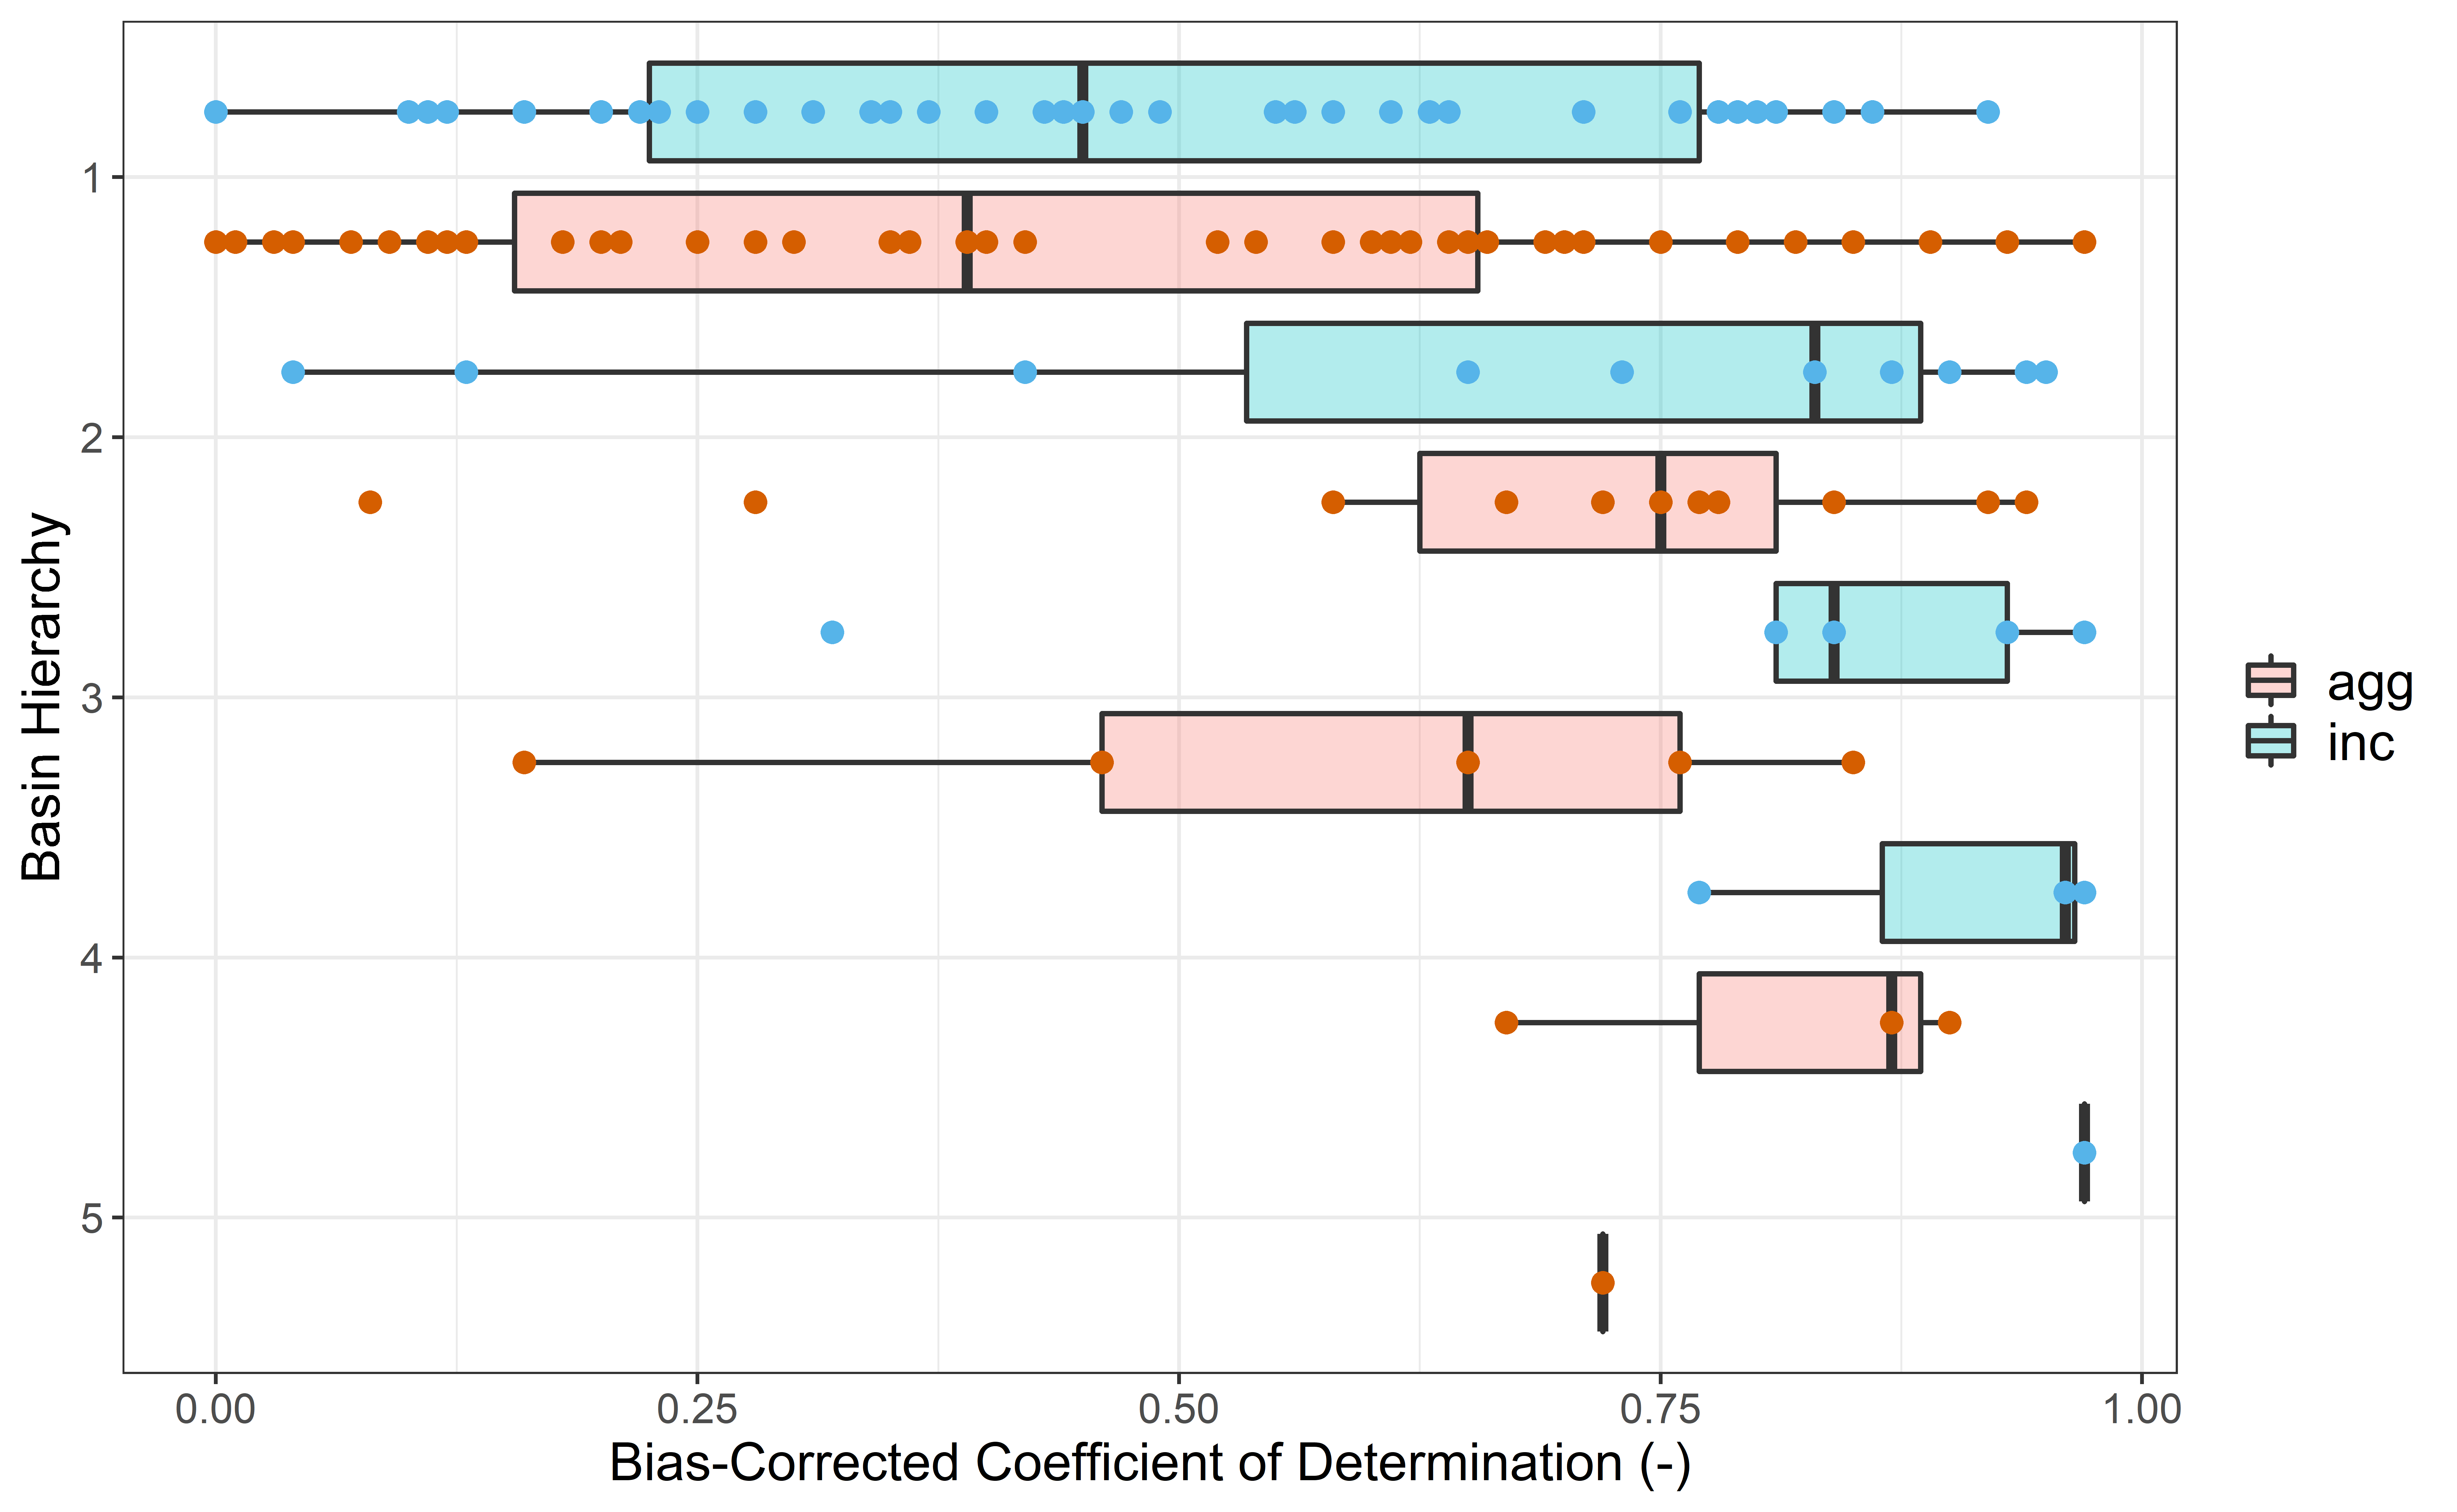
\includegraphics[width=0.8\textwidth, trim={0 0 0 0}, clip=true]{plots/rplot212_bR2gofboxplot_comp.png}
	\caption{The incremental and aggregate basins perform very similarly when there is no information upstream (i.e., hierarchy=1). However, when we introduce information upstream (i.e., hierarchy=2,3,4, and 5) the incremental basins can perform much better than the aggregate.}
	\label{fig:br2boxplotcomp}
\end{figure}

%------------------------------------------------------------------------------------------------------------------------------------------------------------------------
\section{Conclusion}
Incremental basin modeling provides an easy way to include network information in statistical models and the results show that it is valuable for modeling hydrology with parametric models especially those that have a few parameters like the LM and GLM. As the results showed, the LM and GLM prefer the incremental modeling approach, whereas the RF and the NN are somewhat insensitive to it. 

On this data set, and according to the performance ratings provided by \citeA{Moriasi2007885}, the GLM and RF provide a ``good" prediction for unimpaired flows, and the NN provides a ``very good" one (Table \ref{table:modelperformance}). We can hypothesize that the RF performed well due to the nature of non-parametric methods where the model form is determined by the data and hence the data is ``honored" and prediction becomes easier. The NN performance is the best and proves why these methods are so popular in studies in hydroinformatics. 

\begin{table*}[h]\renewcommand{\arraystretch}{1} 
	\linespread{1.0}
	\centering
	\caption{Model performance ratings. Criteria are given by \protect\citeNP{Moriasi2007885} (Appendix \ref{d:mof}).}
	\begin{tabular}{p{5cm}p{5cm}p{5cm}} % must add to 16.5
		\toprule
		Model & Aggregate & Incremental  \\
		\midrule
		LM & Unsatisfactory & Satisfactory \\
		\addlinespace
		GLM & Unsatisfactory & Satisfactory \\
		\addlinespace
		RF & Good & Good \\
		\addlinespace
		NN & Very Good & Very Good \\
		\bottomrule
	\end{tabular}
	\label{table:modelperformance}
\end{table*}

In another experiment, the models were trained on their cumulative flows and cumulative rainfall. Given that snow-melt driven hydrology dominates the Sierra-Nevada basins, and processing the data to its cumulative forms would have given the model a ``memory" effect, we repeated the experiment in this chapter with cumulative values. However, surprisingly, none of the models were able to provide satisfactory results, and therefore, we have therefore left those results out of this chapter. 

The next chapter will explore one flaw we pointed out here: the squared loss function forcing better predictions at flood levels at the expense of drought level data. We will be training models using different asymmetric loss functions to penalize the under predicting of floods and over predicting of droughts at a higher cost (i.e., forcing the model to reach the peaks and valleys of the hydrograph). 

